\pdfoutput=1
\documentclass[11pt]{amsart}
\usepackage{amsmath,amssymb,amsthm}
\usepackage[margin=1.2in]{geometry}
\usepackage{booktabs,adjustbox,graphicx}
\usepackage{xcolor,tikz}
\usetikzlibrary{arrows.meta,calc,positioning}
\usepackage[colorlinks=true,linkcolor=blue,citecolor=blue,urlcolor=blue]{hyperref}
\hypersetup{pdfauthor={Bernd Johannes Wuebben},
 pdftitle={Integral reconstruction and quantitative metric degeneration of K3 bundle moduli}}
\setlength{\emergencystretch}{2em}
\newtheorem{theorem}{Theorem}[section]
\newtheorem{proposition}[theorem]{Proposition}
\newtheorem{lemma}[theorem]{Lemma}
\newtheorem{corollary}[theorem]{Corollary}
\theoremstyle{definition}
\newtheorem{definition}[theorem]{Definition}
\newtheorem{example}[theorem]{Example}
\theoremstyle{remark}
\newtheorem{remark}[theorem]{Remark}
\newcommand{\Z}{\mathbb Z}
\newcommand{\R}{\mathbb R}
\newcommand{\C}{\mathbb C}
\newcommand{\PP}{\mathbb P}
\newcommand{\FF}{\mathbb F}
\newcommand{\OO}{\mathcal O}
\newcommand{\cE}{\mathcal E}
\newcommand{\Q}{\mathcal Q}
\newcommand{\ddbar}{\bar\partial}
\newcommand{\NS}{\operatorname{NS}}
\newcommand{\Ext}{\operatorname{Ext}}
\newcommand{\Hom}{\operatorname{Hom}}
\newcommand{\End}{\operatorname{End}}
\newcommand{\Aut}{\operatorname{Aut}}
\newcommand{\tr}{\operatorname{tr}}
\newcommand{\rank}{\operatorname{rank}}
\newcommand{\im}{\operatorname{im}}
\newcommand{\Vol}{\operatorname{Vol}}
\newcommand{\diam}{\operatorname{diam}}
\newcommand{\coker}{\operatorname{coker}}
\newcommand{\Gr}{\operatorname{Gr}}
\newcommand{\Lie}{\operatorname{Lie}}
\newcommand{\Pic}{\operatorname{Pic}}
\newcommand{\ch}{\operatorname{ch}}
\newcommand{\QQ}{\mathbb Q}
\newcommand{\dis}{\operatorname{dis}}
\newcommand{\supp}{\operatorname{supp}}
\newcommand{\id}{\operatorname{id}}
\title[Integral reconstruction and metric degeneration]{Integral reconstruction and quantitative metric\\ degeneration of K3 bundle moduli}
\author{Bernd Johannes Wuebben}
\subjclass[2020]{14J60 (primary); 14J28, 53C26, 55N35 (secondary)}
\keywords{K3 surface, moduli of bundles, integral cohomology, degeneration,
 harmonic metric, Grassmannian, Gromov--Hausdorff convergence}
\date{November 7, 2026\\This version: November 7, 2026}

\begin{document}
\begin{abstract}
We construct a compact moduli eightfold of rank-seven bundles on a K3
surface whose moving projective lines specialize to Schubert lines in a
deepest Grassmannian fibre \(\Gr(2,4)\). Both middle Schubert classes
extend integrally. The fibre is primitive, has self-intersection six,
and has an explicit degree-eight attachment modulo six. For the natural
\(L^2\) metric defined by harmonic deformation representatives, these
same cycles have exact periods and volumes, ambient diameter asymptotics,
and complete cotangent-Grassmannian rescaled limits. We also prove a
global comparison theorem for compact K3 bundle-moduli contractions
without bubbling, with complete convergent quiver charts whose complex
moment-zero fibres contain simple representations. A principal-stratum
path argument identifies the central harmonic completion, and finite
quotient distances give a variational bound for the distortion of the
actual contraction graph. The bound tends to zero through arbitrary
adjacent chambers. Integral cochains on all geometric overlaps recover
additive cohomology, while universal-index restrictions calculate
middle-degree attachments from a marked complement ring. A mapping-torus
example shows why local fibre rings and divisor classes do not determine
the required monodromy.
\end{abstract}
\maketitle
\section{Introduction}

A contraction remembers an exceptional cycle in several ways.
Its local quotient describes the cycle and its incidence with
neighboring fibres. Its embedding in the compact space determines
integral intersection and attachment data. A degenerating Kähler
metric measures how that same cycle disappears in distance.
The relation between these descriptions is especially concrete
for moduli of bundles on a K3 surface: stable factors determine
a quiver, while universal families identify the quiver's cycles
inside integral cohomology.

This paper joins these descriptions for compact contractions
without bubbling. The central example has a moving projective
line and a deeper Grassmannian fibre \(\Gr(2,4)\).
The line specializes to a Schubert line. The two middle
Schubert classes then reveal information absent from divisor
restrictions: they prove integral primitivity and calculate an
attachment modulo six. On these same cycles, the actual
harmonic metric has exact periods and explicit ambient diameter
asymptotics. A general comparison theorem controls the graph
of the entire compact contraction.

\subsection{The compact Grassmannian example}
The Mukai pairing is
\[
 (r,c,s)\cdot(r',c',s')=c\cdot c'-rs'-r's .
\]
All cohomology and homology in the following statement have
integral coefficients. The harmonic metric is the real,
unnormalized Dolbeault \(L^2\) metric on moduli.

For a universal topological \(K\)-class \(\mathcal E\) on
\(X\times M\), write
\[
 I_z=p_!(z^\vee\otimes\mathcal E),\qquad z\in K^0_{\rm top}(X),
\]
where \(p:X\times M\to M\) and \(p_!\) is the topological
\(K\)-theory pushforward. Thus \(z\) ranges over all integral
topological classes, not only algebraic ones. The marked index-Chern
classes on a complement are the restrictions of \(c_k(I_z)\).
The normalization used below tensors \(\mathcal E\) by the inverse
determinant of a specified rank-one index, as constructed in
Section~\ref{sec:schubert}.

\begin{theorem}\label{thm:main}
There is a projective K3 surface with
\[
 \NS(X)=\Z H\oplus\Z D,\qquad H^2=2,\quad H\cdot D=0,\quad
 D^2=-44,\quad H\text{ ample},
\]
and a unique \(H\)-stable spherical bundle \(A\) of vector
\(a=(3,D,-7)\). Put \(b=(1,0,1)\), \(w=a+b\),
and \(v=2a+b=(7,2D,-13)\).
For sufficiently small generic \(t\ne0\), the entire moduli
space \(M_\pm\) of vector \(v\), for polarization \(H+tD\),
is a smooth compact eightfold of \(K3^{[4]}\) type consisting
of slope-stable bundles. The two chamber spaces have projective
symplectic contractions \(\pi_\pm:M_\pm\to Z\) to a common
normal target with the following properties.

\begin{enumerate}
\item The reduced singular locus is a normal sixfold \(T\)
with one singular point \(o\). Its smooth part parametrizes
classes \(A\oplus F\), where \(F\) is an \(H\)-stable bundle
of vector \(w\); \(o\) represents \(2A\oplus\OO_X\).
The fibres of \(\pi_\pm\) are points, projective lines, and
\(G=\Gr(2,4)\), respectively.
The auxiliary generic \(w\)-moduli resolves \(T\), with
exceptional fibre \(\PP^3\).

\item A moving projective line specializes, in a proper reduced
family, to a minimal Schubert line \(\ell\subset G\).
Every homology inclusion \(H_k(G)\to H_k(M_\pm)\) is primitive,
and \([G]^2=6\). In the positive chamber, let
\(h=c_1(\mathcal U)\), \(p=c_2(\mathcal U)\) for the positive
tautological quotient on \(G\). Normalized universal indices
satisfy
\[
 c(I_z)|_G=(1+h+p)^{\chi(A,z)},\qquad
 \int_Gh^4=2,\quad\int_Gh^2p=\int_Gp^2=1 .
\]
For \(V=M_+\setminus G\), these formulas calculate
\(\kappa:H^8(V)\to\Z/6\) on all marked index-Chern generators,
and
\[
 H^8(M_+)\simeq
 \{(u,N)\in H^8(V)\oplus\Z:\ N\equiv\kappa(u)\pmod6\}.
\]
The marked complement ring remains input to this calculation.

\item Put \(\kappa_t=88\pi|t|/7\).
The minimal line and the moving fibre both have harmonic area
\(\pi\kappa_t\). Either Schubert plane has volume
\((\pi\kappa_t)^2/2\), and \(G\) has volume
\((\pi\kappa_t)^4/12\). Their ambient diameters satisfy
\[
 \diam G=\frac{\pi}{\sqrt2}\sqrt{\kappa_t}(1+O(|t|)),\qquad
 \diam\PP^2=\frac{\pi}{2}\sqrt{\kappa_t}(1+O(|t|)).
\]
The ambient spaces, rescaled by \(\kappa_t^{-1/2}\) and based
on \(G\), converge in complete pointed Gromov--Hausdorff
topology to the unit-level cotangent Grassmannian quotient.
The harmonic metric on \(Z\setminus T\) completes to \(Z\);
the graphs of \(\pi_\pm\) satisfy
Theorem~\ref{thm:quantitative}'s distortion bound and give
compact Gromov--Hausdorff convergence to that completion.
\end{enumerate}
There is no additional non-locally-free or positive-charge
boundary in this compact problem.
\end{theorem}

The local incidence geometry of the Grassmannian is classical.
The point of the theorem is its realization as the entire deep
fibre of this bundle-only compact family, together with its
integral attachment and actual harmonic geometry.
The equal-dimensional incidence resolutions for the two signs
are isomorphic over the affine cone; a nontrivial
Grassmannian flop is not part of the statement.

\subsection{The general reconstruction and metric comparison}
The general hypotheses, stated in
Section~\ref{subsec:hypotheses}, require compact chamber
spaces with a common central slope target, absence of every
ideal boundary, and full convergent quiver charts with a
module-simple point in each complex zero fibre.
The local charts include repeated factors, tangent directions,
inverse solution coverage and the actual classifying maps.

Two kinds of global information enter. For all-degree additive
reconstruction, retain the geometric regular locus and the
local classifying families, with their isomorphism loci.
These determine the actual multiple overlaps and monodromy.
Their integral cochain diagram computes the chamber cohomology
by Proposition~\ref{prop:descent}.
For a compact core \(E\), Theorem~\ref{thm:attachment}
instead uses its intersection map, calculated universal-index
restrictions, and the marked ring of \(M\setminus E\).
Under the stated middle-degree vanishing hypotheses it computes
the boundary homomorphism and an integral fibre product.
These are two useful levels of reconstruction; neither
recovers an unknown global complement from singularity types.

The metric result is quantitative in finite-model distances.
For a sequence of prescribed accuracies we construct finite
covers, positive short-distance scales \(\ell_j\), relative
errors \(\alpha_j\to0\), and variational discrepancies
\(\beta_j(\theta)\to0\) for each fixed \(j\).
If \(R_\theta\) is the graph of the actual contraction, then
\[
 \dis R_\theta\le
 \inf_{j:\theta\in\mathcal P_j}
 \left[\left(\alpha_j+\frac{\beta_j(\theta)}{\ell_j}\right)D_*
                +\beta_j(\theta)\right],
\]
where \(D_*\) is constructed from a fixed central chart cover.
Definitions \eqref{eq:finite-b}--\eqref{eq:global-parameters}
make all these quantities explicit.
The estimate is uniform through stabilizer changes and
arbitrary adjacent-chamber approaches. It is a variational
modulus, rather than a universal power-law rate.

Three points in the proof deserve emphasis.
First, no-charge compactness and local classifying compatibility
put \emph{whole} fibres in the analytic charts.
Second, paths through lower strata can be approximated in
length by paths in the principal stratum; density alone would
not identify the harmonic completion.
Third, first-exit estimates compare both ambient distance
infima, including paths which might leave a local model.
A short-distance correspondence lemma then assembles these
local estimates without using a qualitative global convergence
theorem.

\subsection{Relation to earlier work}
Existence and deformation type of the K3 moduli spaces come
from Yoshioka \cite{yoshioka99,yoshioka01}.
The slope compactifications and the surface comparison with
gauge theory are due to Greb--Toma and
Greb--Sibley--Toma--Wentworth \cite{grebtoma,gstw}.
Quiver descriptions and wall geometry are developed in
Arbarello--Saccà and Bayer--Macrì
\cite{arbarellosacca,bayermacri}.
Grassmannian geometry in K3 moduli also appears in Markman's
Brill--Noether duality \cite{markmanbn}; the present compact
realization is proved from its own rank and charge classification.

The integral generation theorem is Markman's
\cite{markman}, and cochain descent is classical.
Our attachment theorem isolates the elementary relative
argument that turns \emph{calculated} index restrictions into
a boundary homomorphism respecting every integral relation.
The mod-six application uses both Schubert directions; it
does not claim a new presentation of Grassmannian cohomology.
Kaplan--Schedler \cite{kaplanschedler} study compatibility
and monodromy in gluing crepant resolutions.
Here existing compact chamber spaces and their geometric
classifying data are hypotheses; our cochain construction
retains, rather than solves for, their monodromy.

The qualitative formality theorem of
Bandiera--Manetti--Meazzini \cite{bmm} already applies to the
common-slope direct sums used here because their automorphism
groups are reductive. The controlled convergent symplectic
coordinates are imported from \cite{wuebben17}.
Relative finite balancing, complete quotient continuity,
normal slices and the harmonic comparison are imported from
\cite{wuebben14,wuebben15}; their hypotheses and normalizations
are restated in Section~\ref{sec:data}.
The complete cotangent model metric is classical
\cite{biquardgauduchon}.
Our metric contribution is the whole-fibre and principal-path
argument, the explicit global graph bound, and its application
to these identified compact cycles.
Quantitative comparison results such as
Lakzian--Sormani \cite{lakziansormani,lakziansormanier}
place ambient distance discrepancies among their inputs;
we derive the discrepancies here from finite quotient models.
The established qualitative Ricci-flat degeneration theory
\cite{tosatti,song} provides context, but is not an input to
Theorem~\ref{thm:quantitative}.

Sections~\ref{sec:integral}--\ref{sec:global} prove the general
statements. Sections~\ref{sec:construction}--\ref{sec:cycle-metrics}
prove Theorem~\ref{thm:main} on one compact family.
Section~\ref{sec:examples} recovers the fourfold applications
and uses the same two Schubert classes to exhibit the necessity
of retaining monodromy.

\section{Geometric data and harmonic coordinates}\label{sec:data}

We begin by specifying the contraction problems under consideration.
The hypotheses distinguish the geometry needed to identify a compact
moduli space from the local estimates needed to control its metric.
They will be verified, including the entire ideal boundary, for the
eightfold constructed in Section~\ref{sec:construction}.

\subsection{Conventions}
For a projective K3 surface \(X\), write
\[
 v(F)=\ch(F)\sqrt{\operatorname{td}_X}=(r,c,s),\qquad
 ((r,c,s),(r',c',s'))=c\cdot c'-rs'-r's .
\]
Here and below \(\ch\) denotes the Chern character. We fix the
holomorphic determinant. For a smooth family of Ricci-flat Kähler forms
\(\omega_\theta\), set
\(\deg_\theta F=c_1(F)\cdot[\omega_\theta]\) and
\(\mu_\theta(F)=\deg_\theta F/\rank F\).
The harmonic metric is the real part of the \(L^2\) Hermitian pairing
on harmonic \((0,1)\)-deformations, without division by the volume of
\(X\). In particular it is half the real connection convention.

If \(\mathcal E\) is a universal topological \(K\)-class and
\(p:X\times M\to M\), our Mukai homomorphism and family indices are
\begin{equation}\label{eq:mukai-convention}
 \theta_v(z)=\bigl[p_*(\ch(\mathcal E)\sqrt{\operatorname{td}_X}\,z^\vee)\bigr]_2,
 \qquad
 I_z=p_!(z^\vee\otimes\mathcal E),\qquad
 \chi(F,z)=-(v(F),v(z)).
\end{equation}
For \(\theta_v\) the argument belongs to \(v^\perp\); the notation
\(z^\vee\) reverses its degree-two component. A class on \(X\) in a
family-index expression is pulled back without further notation.
Base line bundles may change \(\mathcal E\); they do not change
\(\theta_v|_{v^\perp}\).
The Kähler form of the actual harmonic metric has class
\begin{equation}\label{eq:harmonic-class}
 [\Omega_\theta]=2\pi^2\theta_v(b_\theta),\qquad
 b_\theta=\left(0,[\omega_\theta],
       \frac{c_1(v)\cdot[\omega_\theta]}{\rank v}\right).
\end{equation}
This is the fixed-determinant Chern--Weil formula
\cite[Proposition~4.3, (4.6)]{biswasschumacher} in the real Dolbeault
normalization. Indeed, with
\(\Delta(\mathcal E)=c_2(\mathcal E)-(r-1)c_1(\mathcal E)^2/(2r)\),
that formula reads
\(\omega_{\rm WP}/(2\pi^2)=2p_*(\Delta(\mathcal E)\omega_\theta)\).
Our form is \(\omega_{\rm WP}/2\), and expansion of
\eqref{eq:mukai-convention} gives \eqref{eq:harmonic-class}.
The computation is valid for local twisted families because their
endomorphism bundles are untwisted.

\subsection{The class of contractions}\label{subsec:hypotheses}
Fix an ample central class \(H=[\omega_0]\), a primitive positive-rank
Mukai vector \(v\), and the smooth finite-dimensional family
\(\omega_\theta\). We impose the following three hypotheses.

\medskip\noindent
\textbf{(G1) Compact chamber spaces.}
There are finitely many adjacent chambers and a connected normal
projective variety \(Z\). For all sufficiently small generic parameters,
the full moduli space \(M_\theta\) of slope-stable bundles is smooth
and projective and is also the generic Gieseker moduli space.
There is a proper surjective morphism
\(\pi_\theta:M_\theta\to Z\), constant as a complex morphism within
each chamber. Points of \(Z\) are the \(H\)-polystable classes of
vector \(v\). Every chamber object is \(H\)-semistable, and
\(\pi_\theta\) assigns its \(H\)-graded class. The \(H\)-stable locus
\(U\subset Z\) is connected and dense, and \(\pi_\theta\) is an
isomorphism over \(U\). Fix a finite Whitney stratification refining
the stable-factor decomposition types. The projective and fixed-\(H\)
gauge topologies on \(Z\) agree.

\medskip\noindent
\textbf{(G2) Absence of an ideal boundary.}
Every central ideal Hermitian--Yang--Mills object of vector \(v\) has
zero lost charge, and every \(H\)-semistable sheaf of that vector is
locally free. Thus surface gauge compactness, with the smoothly varying
background forms, has no concentration.

\medskip\noindent
\textbf{(G3) Full convergent quotient models.}
For each central class
\[
 E_p=\bigoplus_i F_i\otimes\C^{m_i},
\]
the full doubled Ext-quiver complex moment zero fibre contains a
module-simple representation of the specified dimension vector.
Here module-simple means that there is no nonzero proper submodule.
All loops, multiplicities and trivial tangent directions are retained.
The convergent symplectic coordinates give local classifying
identifications compatible with the central graded class and the
coarse analytic germ of \(Z\). In these germs,
\begin{equation}\label{eq:classifying-diagram}
 \pi_\theta f_{p,\theta}=f_{p,0}q_{p,\theta},
\end{equation}
where \(q_{p,\theta}\) is the projective quotient map to the affine
zero quotient. This is initially a statement about germs, not about
the full preimage of a target neighborhood.

\medskip
The analytic ingredients in (G3) have precise hypotheses. The
common-slope normal form
\cite[Proposition~2.1]{wuebben17} applies to locally free
\(H\)-polystable bundles on a Ricci-flat K3, with arbitrary ranks and
multiplicities. It is a convergent equivariant holomorphic change
\(\Psi(x)=x+O(\|x\|^3)\), \(D\Psi=I+O(\|x\|^2)\), identifying the
full obstruction ideal with the complex moment ideal.
The resulting harmonic comparison
\cite[Corollary~2.2]{wuebben17}, obtained from the local harmonic
reduction \cite[Theorem~1.1 and Sections~3,5]{wuebben15} and
finite balancing \cite[Theorem~2.1]{wuebben14}, gives
\begin{equation}\label{eq:relative}
 (1-e_p)g_{p,\zeta_p(\theta)}
 \ \leq\ f_{p,\theta}^*g_\theta\
 \leq (1+e_p)g_{p,\zeta_p(\theta)},\qquad
 e_p=C_p(|\theta|+\|x\|^2).
\end{equation}
The inequalities concern tangents to actual smooth quotient pieces.
The local theorem also covers all sufficiently nearby actual solutions.

The finite quotient metric in \eqref{eq:relative} is induced by the
central harmonic norm on \(\Ext^1(E_p,E_p)\). Its real moment covector,
paired by ordinary multiplicity trace, is
\begin{equation}\label{eq:levels}
 \zeta_{p,i}(\theta)=2\pi\bigl(r_i\mu_\theta(v)-\deg_\theta F_i\bigr),
 \qquad \sum_i m_i\zeta_{p,i}=0,\qquad r_i=\rank F_i.
\end{equation}
The compact group is \(\prod_iU(m_i)\), modulo the ineffective common
scalar. The rank weights instead occur in the spectral mass
\(\Vol(\omega_0)\sum_i r_i\tr(\xi_i^*\xi_i)\), whose small quadratic
form is \(\|[\xi,x]\|^2\). These are different pairings.
Constants in \eqref{eq:relative} depend on the fixed background and
its complementary elliptic gaps. They do not depend on ratios of
positive finite eigenvalues or on a nearby stabilizer. Formal
quadraticity alone would not give this estimate; the controlled
convergent coordinates are essential.

\subsection{What the reconstruction retains}\label{subsec:retained}
Retain \(U\) as a geometric space with its interpretation by stable
bundles and local classifying families. Retain also the quotient
domains with their actual families in this same moduli problem.
On two domains, their overlap is the locus of pairs representing
isomorphic bundles. Injective coarse classifying maps identify its
two projections with open subsets and give a unique transition map.
We take cochains only after these overlap spaces and maps have
been specified. In particular a bare cochain complex of \(U\) is not
enough to define the overlaps.

These geometric maps retain stratum monodromy and all multiple
compatibilities. Local fibre types alone do not supply them.
Specialization of exceptional classes will be computed from a
separate proper family in Section~\ref{subsec:specialization}.
For the smaller middle-degree calculation, the global datum is
instead the marked ring \(H^*(M\setminus E,\Z)\), where \(E\) is the
chosen compact exceptional core. This complement generally contains
exceptional fibres over other strata. In our eightfold it is larger
than \(\pi^{-1}(U)\).

\section{Integral attachment and cochain descent}\label{sec:integral}

The useful reduction in the middle degree is elementary once the
correct integral restrictions have been calculated. We state it
first, so that the later Grassmannian computation has a definite
target: the homomorphism \(\kappa\), not just its finite codomain.

\subsection{A calculated boundary homomorphism}
Let \(M\) be a closed oriented smooth \(2n\)-manifold and \(E\subset M\)
a compact tame subset. Suppose it has a closed oriented regular
neighborhood \(W\) retracting onto \(E\), with smooth boundary \(L\).
Put \(V=M\setminus E\). Collars identify the overlap of \(V\) with an
open neighborhood of \(E\), up to homotopy, with \(L\).
Assume
\begin{equation}\label{eq:attachment-assumptions}
 \begin{gathered}
 H_n(E,\Z)=\Lambda\ \text{is free},\qquad H^n(E,\Z)=\Lambda^*,\\
 H^{n-1}(E,\Z)=H_{n-1}(E,\Z)=0,\qquad
 B:\Lambda\longrightarrow\Lambda^*\ \text{is injective}.
 \end{gathered}
\end{equation}
Here the dual identification is evaluation, and \(B\) is the middle
intersection map in \(W\). Let \(C=\coker B\).

\begin{theorem}\label{thm:attachment}
Suppose homogeneous integral classes \(g_j\in H^*(M,\Z)\) have
degree-\(n\) monomials generating \(H^n(M,\Z)\).
Supply the ring \(A=H^*(V,\Z)\) with the distinguished classes
\(a_j=g_j|_V\), and calculate \(r_j=g_j|_E\).
Then \(H^{n-1}(L,\Z)=0\), \(H^n(L,\Z)=C\), and
\begin{equation}\label{eq:kappa}
 \kappa\bigl(P(a_j)\bigr)=[P(r_j)]\in C
\end{equation}
is a well-defined homomorphism on all of \(A^n\).
It is the actual boundary restriction and gives
\begin{equation}\label{eq:fibre-product}
 H^n(M,\Z)\ \simeq\
 \{(u,z)\in A^n\oplus\Lambda^*:\ \kappa(u)=[z]\text{ in }C\}.
\end{equation}
The isomorphism is restriction to \(V\) and \(W\).
\end{theorem}

\begin{proof}
Poincaré--Lefschetz duality and the sequence of \((W,L)\) give
\[
 0\longrightarrow H^{n-1}(L,\Z)\longrightarrow\Lambda
 \xrightarrow{B}\Lambda^*\longrightarrow H^n(L,\Z)
 \longrightarrow0.
\]
This proves the boundary assertions. Excision also gives
\(H^{n+1}(M,V;\Z)=H_{n-1}(E,\Z)=0\).
Therefore restriction \(H^n(M,\Z)\to A^n\) is onto, and the
monomials in the \(a_j\) generate \(A^n\).

It remains to check every relation, which is the point of the
formula. If \(P(a_j)=0\), the class \(P(g_j)\) comes from
\(H^n(M,V;\Z)=\Lambda\). Its restriction to \(W\) is the image of
that same element under \(B\). Hence \(P(r_j)\in B\Lambda\),
so \eqref{eq:kappa} is independent of its polynomial representative.
The two restrictions of each \(g_j\) agree on \(L\); consequently
\(\kappa\) is the boundary restriction. The Mayer--Vietoris sequence,
with \(H^{n-1}(L,\Z)=0\), now identifies \(H^n(M,\Z)\) with the
kernel of \((u,z)\mapsto\kappa(u)-[z]\).
\end{proof}

This is an integral fibre product. It retains the finite boundary
group, saturation and extension information that would disappear
after tensoring with \(\QQ\). It requires the marked complement ring;
it does not calculate that ring from the singularity. A basis change
in \(\Lambda\) gives the naturally isomorphic fibre product.
Changing the generating set changes the formula, but not the
homomorphism, because it is the same boundary restriction.
Isotopic regular neighborhoods give the same result under collar
identifications.

\subsection{Integral generators from universal indices}
For primitive-vector K3 moduli, the required global generators come
from \eqref{eq:mukai-convention}. Markman's theorem
\cite[Theorem~1]{markman} states that Chern classes of the topological
\(K\)-theory Künneth factors of a universal class generate integral
cohomology. The integral Euler pairing on \(K^0_{\rm top}(X)\) is
perfect. Taking an Euler-dual integral basis therefore expresses
those factors as the indices \(I_z\). Thus the classes \(c_k(I_z)\)
generate \(H^*(M,\Z)\). The same theorem gives odd vanishing and
torsion-freeness in this K3 setting.

Both qualifications matter: all topological \(K\)-classes are
allowed, and the generation is integral. Algebraic indices alone,
or rational Chern characters alone, would not justify
Theorem~\ref{thm:attachment}. In a concrete exceptional family,
a base-line ambiguity can often be removed by the determinant of a
rank-one global index. Section~\ref{sec:schubert} performs exactly
this normalization before calculating \(\kappa\).

\subsection{All degrees and all overlaps}\label{subsec:cochains}
The general construction uses the geometric data of
Section~\ref{subsec:retained}. Whole-fibre coverage, proved in
Proposition~\ref{prop:coverage}, supplies a finite open cover
\(\mathcal U=(U_i)\) of \(M_\theta\) by those domains, together with
domains in the regular locus. Write \(U_I=\bigcap_{i\in I}U_i\).
Every intersection is expressed in any one of its coordinates by
the actual classifying transitions.

\begin{proposition}\label{prop:descent}
Let
\[
 K^{p,q}(\mathcal U)=
 \prod_{i_0<\cdots<i_p} C^q(U_{i_0\cdots i_p};\Z).
\]
With alternating restriction differential \(\delta\) and total
differential \(D=\delta+(-1)^p d\), restriction induces a
quasi-isomorphism
\begin{equation}\label{eq:cech}
 C^*(M_\theta;\Z)\longrightarrow\operatorname{Tot}K(\mathcal U).
\end{equation}
Changing the cover, slices or family trivializations gives the same
object in the derived category of integral complexes.
\end{proposition}

\begin{proof}
The coarse coordinate maps are unique on their overlaps and hence
satisfy the cocycle identity on triples, and all its higher
consequences. Thus \(D^2=0\).

Use first the singular chains subordinate to \(\mathcal U\).
Barycentric subdivision and its usual chain homotopy show that their
inclusion in all singular chains is a chain-homotopy equivalence.
For each subordinate simplex, the set of indices of cover members
containing its image is a nonempty simplex. Its augmented Čech
complex is contractible. Taking the corresponding products proves
exactness of the augmented cochain resolution in the Čech direction.
The Čech degree is bounded because the cover is finite; its
filtration gives \eqref{eq:cech}.

A refinement commutes with augmentation, so its total-complex map
is a quasi-isomorphism. Two covers have a common intersection
refinement. Different refinement assignments induce the same map
in the derived category, since both commute with the invertible
augmentation from \(C^*(M_\theta;\Z)\). Finally a change of slices
or trivializations conjugates the overlap diagram by the unique
coarse coordinate maps. Base-line twists, and different presentations
of a universal gerbe, do not change those coarse maps.
\end{proof}

The descent assertion is classical; compare the open-cover
construction in \cite[Section~4G]{hatcher}. Its application here uses the
geometric identification of the domains and their overlaps, rather
than replacing them by lists of fibre cohomology groups.
The complex retains all multiple intersections and monodromy.
It computes additive integral cohomology; no cup-product or
homotopy-type assertion is being inferred from this additive
statement. A finite cover gives a finite diagram of complexes,
not automatically a finite matrix calculation. Compatible cellular
models can make it finite when their maps are also supplied.

In particular, the formal descent argument does not solve the
existence or compatibility problem for arbitrary local resolutions.
The local-to-global theory of Kaplan--Schedler
\cite{kaplanschedler} treats such compatibility and monodromy
questions in a broader setting. Here the compact projective
chamber spaces are already part of (G1). Our task is to identify
whole local fibres within them and to calculate the integral
attachments on their universal-index classes.

\section{Paths through the principal stratum}\label{sec:paths}

Before comparing compact spaces, we identify the central metric that
will be their limit. Density of the stable locus is not sufficient:
a dense Riemannian stratum can have a larger intrinsic distance.
We prove equality of distances by perturbing paths and controlling
the short joins between their pieces.

\subsection{Short paths in a fixed semialgebraic set}
We use the following elementary consequence of semialgebraic
triangulation and uniform monotonicity
\cite[pp.~116,130,133]{vandendries}.

\begin{lemma}\label{lem:bounded-paths}
A nonempty bounded connected semialgebraic set \(S\subset\R^N\),
not necessarily closed, has finite intrinsic diameter for
Euclidean path length. More precisely, every two points can be
joined in \(S\) by a continuous semialgebraic path of length at
most a constant \(C_S\).
\end{lemma}

\begin{proof}
Triangulate the compact closure compatibly with \(S\).
Its inverse image is a finite union of relative open simplices.
Choose their barycenters and connect two when one included simplex
is a face of the other. The connecting segment lies in the larger
open simplex except at its endpoint and stays in the union.
The resulting finite incidence graph is connected. Otherwise one
component and its complement would be relatively open and closed:
a relative limit between included cells can only occur along a
face incidence, which would connect the components.

Choose a spanning tree. Join each variable endpoint to its cell
barycenter and then follow the tree between barycenters. Transport
the resulting polygonal paths through the semialgebraic
triangulation map. There are finitely many endpoint-cell choices,
so this is a semialgebraic family of continuous paths. Cell decomposition and uniform finiteness, applied with the two
endpoints as parameters, bound the number of monotonicity intervals
of each coordinate by a common integer. Every coordinate stays in the
bounded range of \(S\). The sum of its coordinate variations
therefore gives a uniform finite bound for path length.
\end{proof}

For a positive-dilation-invariant set, applying the lemma in its
unit ball gives joining paths of length \(C_S\rho\) in its
radius-\(\rho\) ball. This is a statement about a fixed set; it
does not assert a uniform constant for arbitrary degenerating
families.

\subsection{The simple zero quotient}
Let \(W\) be a full doubled-quiver representation, with compact
group \(K\) a connected product of unitary groups modulo an
ineffective common scalar. Put
\[
 A_0=\{\mu_{\C}=0,\ \mu_{\R}=0\},\qquad Q_0=A_0/K.
\]
Assume that the complex zero fibre contains a module-simple
representation. Write \(A_0^s\) for the balanced simple locus and
\(Q_0^s=A_0^s/K\).
We use the finite intrinsic theorem
\cite[Section~5]{wuebben14}: \(Q_0\), with the infimum of
finite-stratum path lengths, is a proper geodesic space whose
metric topology is the quotient topology. We also use its full
normal metric slice and normal-simple results
\cite[Sections~4,6]{wuebben14}. These retain the complete normal
representation and require the simple-zero hypothesis.

\begin{lemma}\label{lem:simple-paths}
There is a constant \(C_W\) such that every two points of
\(A_0^s\) of norm at most \(\rho\) can be joined in \(A_0^s\),
within that ball, by a path of length at most \(C_W\rho\).
At any point of \(Q_0\), nearby simple points admit simple joining
paths whose length tends to zero and which stay in any fixed
sufficiently small neighborhood.
\end{lemma}

\begin{proof}
Crawley--Boevey's theorem \cite[Theorem~1.2]{crawleyboevey},
under the existence of a simple representation, makes the complex
zero fibre irreducible and generically simple. Its simple quotient
is a connected smooth open complex variety. Kempf--Ness identifies
this with \(Q_0^s\). The compact-group quotient
\(A_0^s\to Q_0^s\) is proper with connected fibres. A separation
of its source would induce a separation of its target, by the
closed-map property and connected fibres. Hence \(A_0^s\) is connected.

Simplicity is semialgebraic: for each proper subdimension vector,
the existence of invariant subspaces is a polynomial incidence
condition on a product of Grassmannians, followed by projection.
There are finitely many such vectors. The balanced moment equations
are real polynomial, and \(A_0^s\) is invariant under positive
dilation. The map \(x\mapsto x/\max(1,\|x\|)\) retracts it onto its
unit-ball part. That part is connected and bounded, so
Lemma~\ref{lem:bounded-paths} and scaling prove the first assertion.
The zero-dimensional case uses constant paths.

For the second assertion take the full normal slice at a balanced
representative of the chosen point. Its stabilizer is connected,
and its full normal representation again has a module-simple point
by the normal-simple theorem. Representatives of nearby points
tend, after unitary adjustment, to zero in this slice.
A closed zero-level representation has scalar stabilizer exactly
when it is simple; the slice preserves this condition.
Apply the first assertion in the full normal representation.
The bounded metric comparison of the slice takes its \(C\rho\)
joins to joins of length at most \(C'\rho\) in the ambient quotient.
Their images lie in any prescribed fixed neighborhood for small
\(\rho\).
\end{proof}

Projection cannot increase the lengths of the balanced paths.
Semialgebraic paths are piecewise smooth after finite subdivision,
and within the simple stratum they may be smoothed with arbitrarily
small additional length.

\begin{proposition}\label{prop:principal-completion}
The intrinsic Riemannian distance of \(Q_0^s\) equals the restriction
of the full finite-stratum distance of \(Q_0\).
Its metric completion is \(Q_0\).
\end{proposition}

\begin{proof}
One inequality follows because every simple path is admissible
in the full quotient. For the reverse, take simple endpoints and
a finite-stratum path of length within \(\epsilon\) of their full
distance. Truncate an arbitrarily small total length at its finitely
many stratum junctions. Cover the remaining compact smooth pieces
by normal slice charts with relative squared-metric errors less
than a chosen \(\delta>0\), and subdivide.

In a full slice the given stratum is \(T\times\{0\}\), where the
group acts trivially on \(T\). Choose balanced simple normal points
\((u_j,z_j)\to0\). Translation in \(T\) removes \(u_j\), without
changing the moment map or stabilizer. Replace a piece
\((u(t),0)\) by \((u(t),z_j)\). Its product-metric speed is exactly
the old speed. Comparing both curves with that same product metric
increases length by at most
\(\sqrt{(1+\delta)/(1-\delta)}\). Their endpoints converge.

Use Lemma~\ref{lem:simple-paths} to join the perturbed endpoints
at each subdivision point. At an original singular junction,
first choose a neighborhood where the joining cost is below an
assigned tolerance, then truncate far enough toward the junction
to place both endpoints there. Small simple perturbations remain
there. The same construction joins to the original simple endpoints.
There are finitely many joins; allocate their total cost below
\(\epsilon\), and choose the chart errors so their total length
inflation is below \(\epsilon\).
The resulting simple path has length at most the full distance
plus \(3\epsilon\). Let \(\epsilon\downarrow0\).

The simple locus is dense in the quotient topology, hence in the
finite metric topology. Properness gives completeness of \(Q_0\),
so it is the asserted completion.
\end{proof}

This argument explains why lower-dimensional strata create no
new shortcuts between stable points: every such path can be
approximated with its length, not merely with its endpoints.

\section{Whole fibres and quantitative global distances}\label{sec:global}

The local estimates have relative errors, whereas gluing distances
introduces additive errors. We keep these separate. First we obtain
whole-fibre charts and the central completion. We then compare short
ambient pairs in both directions, and finally concatenate geodesics.

\subsection{Coverage and compatibility}
\begin{proposition}\label{prop:coverage}
Under \textup{(G1)--(G3)}, local classifying charts can be chosen to
contain the whole preimages of smaller target neighborhoods, for
all sufficiently small generic parameters. For each prescribed
relative accuracy they give finite covers with that accuracy.
Their coarse transitions satisfy all cocycle identities, and if
two squared-metric errors are \(\epsilon_i,\epsilon_j<1/2\), then
\begin{equation}\label{eq:overlap-metric}
 \frac{1-\epsilon_i}{1+\epsilon_j}g_i
 \le h_{ij,\theta}^*g_j
 \le\frac{1+\epsilon_i}{1-\epsilon_j}g_i .
\end{equation}
\end{proposition}

\begin{proof}
By (G2), a sequence of nearby chamber connections has a subsequence
converging smoothly modulo gauge to a central polystable bundle.
Indeed surface compactness first gives an ideal limit; the
small-energy estimates and removability leave only positive
integral lost charge, which (G2) excludes. The smoothly varying
background metrics and determinant connections preserve these
local estimates; see also \cite[Lemma~3.2]{wuebben17}.

Suppose \(\theta_n\to0\) and \(\pi_{\theta_n}(E_n)\to p\).
Let \(E\) be a smooth gauge subsequential limit.
Inverse coverage in the local solution chart at \(E\) gives
balanced coefficients \(x_n\to0\), after compact-group adjustment.
Equation~\eqref{eq:classifying-diagram} identifies their target
classes with the affine invariants of \(x_n\), which converge
to the vertex at \([E]\). Since \(Z\) is Hausdorff, \([E]=p\).

Fix an outer chart at \(p\). If no smaller target neighborhood
and parameter ball had their whole preimages inside it, choose
points outside the chart with targets tending to \(p\) and
parameters tending to zero. The preceding conclusion puts them
in its open actual solution neighborhood, a contradiction.
Finite invariant properness bounds balanced representatives with
bounded invariants and small levels. Shrinking the target neighborhood
therefore puts its whole preimage in any chosen inner coefficient
ball. Conversely, the finite projective quotient is onto its affine
target, and its small representatives classify actual nearby
bundles. This gives coverage on both sides.

For a prescribed accuracy, shrink an outer chart separately at
each \(p\) using \eqref{eq:relative}. Extract a finite subcover of
their inner target images, and only then shrink the common parameter
ball. This order avoids any claim of a uniform complementary
elliptic gap for separate stable backgrounds approaching a
reducible limit. A chart at the reducible limit covers that region.

On overlaps put \(h_{ij,\theta}=f_{j,\theta}^{-1}f_{i,\theta}\).
These are the unique coarse identifications of the same holomorphic
bundle classes, so they satisfy \(h_{jk,\theta}h_{ij,\theta}
=h_{ik,\theta}\). They are holomorphic in complex coordinates and
smooth on smooth quotient pieces. Comparing each finite metric
with the same actual harmonic metric gives
\eqref{eq:overlap-metric}.
\end{proof}

Universal families on overlapping domains can differ by a base
line or a gerbe presentation. The coarse transition used above is
unaffected. Proposition~\ref{prop:coverage} also supplies the
geometric cover used in Proposition~\ref{prop:descent}.

\subsection{The central length space}
Give each central representation-type stratum its harmonic metric.
Let \(d_0\) be the infimum of the lengths of paths with finitely
many smooth stratum pieces and finite one-sided endpoint lengths.

\begin{proposition}\label{prop:central-completion}
The function \(d_0\) is a metric inducing the projective topology
of \(Z\). It makes \(Z\) a compact geodesic space and is the
completion metric of the intrinsic harmonic metric on \(U\).
A finite upper bound \(D_*\ge\diam(Z,d_0)\) can be constructed
from one finite central chart cover and its coarse metric bounds.
\end{proposition}

\begin{proof}
At zero level the model radius is the distance to the cone vertex.
Small model neighborhoods thus connect nearby points at cost
bounded by a fixed multiple of their radii. The local tensor
comparison transfers these paths to \(Z\). Connectedness and a
finite chart cover make all distances finite.

There is also a lower bound for leaving a chart. With squared
metric comparison between \(1/2\) and \(2\), a path beginning at
model radius \(r<R\) and leaving the radius-\(R\) sublevel has
length at least
\begin{equation}\label{eq:exit}
 (R-r)/\sqrt2 .
\end{equation}
The model radius is 1-Lipschitz, and the image of a closed sublevel
is compact, so a first exit must meet its radial boundary.
This applies to ambient paths, without assuming that their later
portions remain in the chart. Local finite metric lower bounds,
together with \eqref{eq:exit}, separate distinct points.
The short local paths give the reverse topological continuity.
Thus \(d_0\) induces precisely the topology of \(Z\).
Projective compactness gives metric compactness; the path definition
makes it a length metric and hence a geodesic metric.

Apply the perturbation proof of
Proposition~\ref{prop:principal-completion} to a finite subdivision
of a central actual path. Both the original and perturbed curves
are compared with the same local model, using arbitrarily small
relative errors. The simple joins have arbitrarily small total
cost. Therefore the intrinsic distance on \(U\) is \(d_0|_U\).
Density and compactness identify its completion with \(Z\).

For the last assertion choose a finite cover by connected inner
radial neighborhoods with coarse comparison at most \(2\).
Its intersection graph is connected. Choose an overlap point for
each edge in a spanning tree. Within a chart, join its center
and these points through its cone vertex, with length bounded by
its radius times the coarse comparison factor. A simple tree path
visits each chart at most once. The sum of these finitely many
local bounds, including the two endpoint joins, is a permissible
\(D_*\). No unknown global distance enters this construction.
\end{proof}

\subsection{Finite-model discrepancies}
Fix a central chart \(p\), and write \(Q_\zeta\) for its complete
finite quotient, \(d_\zeta\) for its intrinsic metric, \(r_\zeta\)
for the norm of a balanced representative, and
\(q_\zeta:Q_\zeta\to Q_0\) for the projective quotient map.
For \(r>0\), define
\begin{align}
 b_{p,r}(\theta)
 &=\sup_{\substack{q_\zeta(x)=z,\ q_\zeta(x')=z'\\
                         r_0(z),r_0(z')\le r}}
       |d_\zeta(x,x')-d_0(z,z')|,\label{eq:finite-b}\\
 a_{p,r}(\theta)
 &=\sup_{\substack{q_\zeta(x)=z\\r_0(z)\le r}}
       |r_\zeta(x)-r_0(z)|,\qquad
 \widetilde a_{p,r}(\theta)
 =\sup_{r_\zeta(x)\le r}|r_0(q_\zeta(x))-r_\zeta(x)|,
 \label{eq:finite-a}
\end{align}
where \(\zeta=\zeta_p(\theta)\); the \(d_0\) in
\eqref{eq:finite-b} is the finite zero-model distance.
We distinguish it from the central global distance by its arguments.

\begin{lemma}\label{lem:discrepancies}
The three quantities in \eqref{eq:finite-b}--\eqref{eq:finite-a}
are finite and tend to zero as \(\theta\to0\).
\end{lemma}

\begin{proof}
Properness of the projective quotient and finite invariant
properness bound balanced representatives uniformly for small
levels and bounded target radii. The source-radius condition
already gives bounded representatives in the other supremum.
All relevant sets are compact.

If one convergence failed, take a contradicting sequence and
convergent subsequences of its balanced representatives.
Source and target have the same affine invariants. At zero level
uniqueness of the balanced orbit identifies their limits.
Continuity of radius proves the two radial assertions. Finite
intrinsic parameter continuity
\cite[Theorem~5.1]{wuebben14}, applied to the two pairs of
representatives, proves the distance assertion. There are finitely
many parameter faces; passage to a face subsequence covers all
approaches.
\end{proof}

These are variational functions of specified finite moment equations,
norms and path distances. No semialgebraicity of those distances
is required. The two radial functions serve different purposes:
one bounds the preimage of a target ball, the other the image of
a source ball.

\subsection{From short pairs to global distortion}
For a correspondence \(R\subset X\times Y\), write
\[
 \dis R=\sup_{(x,y),(x',y')\in R}
          |d_X(x,x')-d_Y(y,y')|.
\]

\begin{lemma}\label{lem:short-correspondence}
Let \(X,Y\) be nonempty compact length spaces and \(R\) a
correspondence. Suppose \(\ell>0\), \(\alpha,\beta\ge0\), and
\[
 \begin{aligned}
 d_X(x,x')\le\ell&\ \Longrightarrow\
 d_Y(y,y')\le(1+\alpha)d_X(x,x')+\beta,\\
 d_Y(y,y')\le\ell&\ \Longrightarrow\
 d_X(x,x')\le(1+\alpha)d_Y(y,y')+\beta
 \end{aligned}
\]
for all related pairs. With \(D=\diam X\) and
\(q=\alpha+\beta/\ell\), one has
\begin{equation}\label{eq:short-bound}
 \dis R\le qD+\beta,\qquad
 d_{\rm GH}(X,Y)\le\tfrac12(qD+\beta),\qquad
 \diam Y\le(1+q)D+\beta .
\end{equation}
\end{lemma}

\begin{proof}
Subdivide an \(X\)-geodesic of positive length \(d_X(x,x')\)
into \(N=\lceil d_X(x,x')/\ell\rceil\) segments. Choose arbitrary
related \(Y\)-points at the interior division points and the
prescribed endpoints. Summing gives
\(d_Y(y,y')\le(1+q)d_X(x,x')+\beta\).
For zero \(X\)-distance the local inequality gives this directly.
Interchanging \(X,Y\) gives the reverse global inequality.
If \(d_Y\ge d_X\), their difference is at most \(qd_X+\beta\le qD+\beta\).
If \(d_X\ge d_Y\), it is at most \(qd_Y+\beta\le qD+\beta\).
This proves the distortion estimate, and the other assertions
follow from the correspondence bound and the first global inequality.
\end{proof}

We now specify every quantity in the global bound. Choose
\(0<\epsilon_j\downarrow0\), with \(\epsilon_j<1/8\).
At each central point choose an outer coefficient radius \(16r\)
where the central error in \eqref{eq:relative} is at most
\(\epsilon_j/2\). Extract a finite cover by central radius-\(r/4\)
images; write its radii as \(r_{ji}\).
After that choice, shrink a parameter neighborhood \(\mathcal P_j\)
so the nearby outer errors are at most \(\epsilon_j\), whole-preimage
coverage holds, and
\[
 a_{i,r_{ji}},\ \widetilde a_{i,r_{ji}}<r_{ji}/16,
 \qquad b_{i,r_{ji}}<r_{ji}.
\]
Choose any
\begin{equation}\label{eq:global-parameters}
 \begin{gathered}
 0<\ell_j<\min_i\frac{r_{ji}}{16\sqrt2},\qquad
 \alpha_j=\sqrt{\frac{1+\epsilon_j}{1-\epsilon_j}}-1,\\
 \beta_j(\theta)=\sqrt{1+\epsilon_j}\,
                  \max_i b_{i,r_{ji}}(\theta).
 \end{gathered}
\end{equation}

\begin{figure}[tb]
 \centering
 \resizebox{\linewidth}{!}{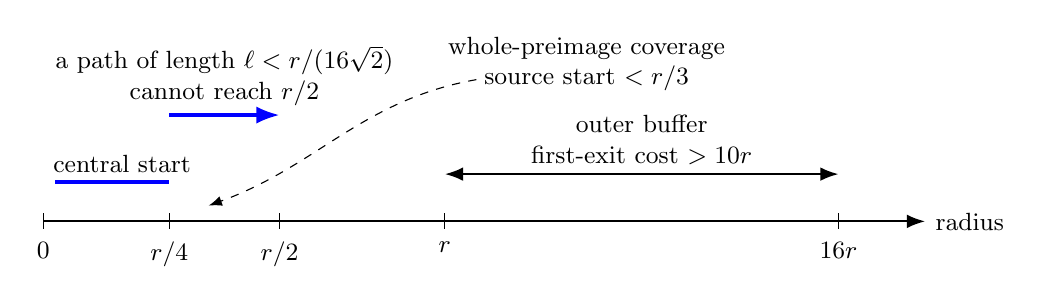
\begin{tikzpicture}[>=Latex,every node/.style={font=\small}]
 \draw[thick,->] (0,0) -- (11.2,0) node[right] {radius};
 \foreach \x/\lab in {0/0,1.6/{r/4},3/{r/2},5.1/r,10.1/{16r}} {
  \draw (\x,.1)--(\x,-.1);
  \node[below=4pt] at (\x,0) {\(\lab\)};
 }
 \draw[very thick,blue] (.15,.5) -- (1.6,.5);
 \node[above] at (1,.5) {central start};
 \draw[very thick,blue,->] (1.6,1.35) -- (3,1.35);
 \node[above,align=center] at (2.3,1.35)
    {a path of length \(\ell<r/(16\sqrt2)\)\\cannot reach \(r/2\)};
 \draw[thick,<->] (5.1,.6) -- (10.1,.6);
 \node[above,align=center] at (7.6,.6)
    {outer buffer\\first-exit cost \(>10r\)};
 \node[align=center] at (6.9,2.0)
    {whole-preimage coverage\\source start \(<r/3\)};
 \draw[dashed,->] (5.5,1.8) to[out=190,in=20] (2.1,.2);
\end{tikzpicture}
}
 \caption{The radius buffers for one chart, schematically and
 not to scale. A short pair starts in the central \(r/4\)
 ball and remains in the range where both finite discrepancies
 apply. The outer \(16r\) chart excludes ambient shortcuts.
 The source start bound uses \(a_r\); the reverse transfer
 of its endpoint uses \(\widetilde a_r\).}
 \label{fig:buffers}
\end{figure}

\begin{theorem}\label{thm:quantitative}
Under \textup{(G1)--(G3)}, let \(R_\theta\) be the graph of
\(\pi_\theta\), with the harmonic distance on \(M_\theta\) and
the completion distance on \(Z\). Then
\begin{equation}\label{eq:global-distortion}
 \dis R_\theta\le
 \inf_{j:\,\theta\in\mathcal P_j}
 \left[\left(\alpha_j+\frac{\beta_j(\theta)}{\ell_j}\right)D_*
              +\beta_j(\theta)\right].
\end{equation}
For each fixed \(j\), \(\mathcal P_j\) contains all sufficiently
small generic parameters and \(\beta_j(\theta)\to0\).
The right side tends to zero through arbitrary adjacent chambers.
Consequently \((M_\theta,d_\theta)\) converges in compact
Gromov--Hausdorff topology to the harmonic completion \((Z,d_0)\).
\end{theorem}

\begin{proof}
Fix \(j\) and one of its charts, and abbreviate \(r=r_{ji}\),
\(\epsilon=\epsilon_j\). First suppose both central endpoints have
model radius at most \(r\). Their finite central distance is at
most \(2r\), by joining through the cone vertex. Their finite
source distance is at most \(2r+b<3r\), and source radii are
at most \(r+a<17r/16\).
Finite near-minimizers stay inside the radius-\(16r\) chart,
because radius is 1-Lipschitz. Their actual images give competitors
of length less than \(4r\). On the other hand, any actual path
leaving that outer chart pays more than \(10r\) before its first
exit, by \eqref{eq:exit}. The closed sublevel images and
whole-preimage coverage justify this barrier for ambient paths.
Thus taking infima in both directions gives
\begin{equation}\label{eq:local-ambient}
 \begin{aligned}
 d_\theta(x,x')&\le(1+\alpha_j)d_0(\pi_\theta x,\pi_\theta x')
                         +\beta_j(\theta),\\
 d_0(\pi_\theta x,\pi_\theta x')
              &\le(1+\alpha_j)d_\theta(x,x')+\beta_j(\theta).
 \end{aligned}
\end{equation}
The relative factor compares the two squared-metric errors;
the larger required additive factor is \(\sqrt{1+\epsilon}\,b\).

It remains to put every short ambient pair in such a chart.
Choose an inner radius-\(r/4\) chart containing \(\pi_\theta x\).
Its entire source preimage has radius at most \(5r/16<r/3\).
If the central distance to \(\pi_\theta x'\) is at most \(\ell_j\),
a central near-minimizer cannot reach radius \(r/2\): its exit
cost is at least \(r/(4\sqrt2)>\ell_j\).
Hence the other target endpoint is inside radius \(r/2\).
If instead the source distance is at most \(\ell_j\), the source
exit cost from radius at most \(r/3\) to radius \(r/2\) is at least
\(r/(6\sqrt2)>\ell_j\). Thus \(x'\) has source radius less than
\(r/2\). The function \(\widetilde a\) then puts its target
inside radius \(r\). In either case both inequalities
\eqref{eq:local-ambient} apply.

Use Lemma~\ref{lem:short-correspondence} with
\(X=(Z,d_0)\), \(Y=(M_\theta,d_\theta)\), and the transposed
graph of \(\pi_\theta\). Both spaces are compact length spaces
and \(\diam X\le D_*\) by
Proposition~\ref{prop:central-completion}.
This proves the expression in brackets for each admissible \(j\).
Taking its infimum proves \eqref{eq:global-distortion}.

For fixed \(j\), the finite discrepancy lemma gives
\(\beta_j(\theta)\to0\). Therefore the limit superior of the
bound is at most \(\alpha_jD_*\). Now let \(j\to\infty\).
The correspondence estimate in \eqref{eq:short-bound} proves
the stated convergence.
\end{proof}

The construction first fixes accuracy, then selects a finite
cover, then takes the parameter limit. It gives an explicit
variational modulus, with no assertion of a universal power law.
In particular it does not use qualitative global
Gromov--Hausdorff convergence as a premise.

\section{A compact contraction with Grassmannian fibre}\label{sec:construction}

We now construct a family for which the general statements have
two independent Schubert directions to detect.
Its central repeated factor has multiplicity two, so its effective
local group is \(U(2)\). The construction includes the full compact
moduli spaces, not only the Grassmannian quotient near one point.

\subsection{The surface and the complete factor list}
Choose a K3 surface with
\begin{equation}\label{eq:rankseven-lattice}
 \NS(X)=\Z H\oplus\Z D,\qquad H^2=2,\quad H\cdot D=0,\quad D^2=-44.
\end{equation}
Such a surface exists: the primitive embedding
\(H=e_1+f_1,\ D=e_2-22f_2\) into two hyperbolic planes and
Morrison's realization theorem
\cite[Corollary~2.9(i)]{morrison} give the full Néron--Severi
lattice. A root would satisfy \(h^2-22m^2=-1\), impossible modulo
eleven. We choose the positive component so that \(H\) is ample.
Put
\begin{equation}\label{eq:rankseven-vectors}
 a=(3,D,-7),\quad b=(1,0,1),\quad
 w=a+b=(4,D,-6),\quad v=2a+b=(7,2D,-13).
\end{equation}
Then
\[
 a^2=b^2=-2,\quad(a,b)=4,\quad w^2=4,\quad v^2=6,\quad
 (a,w)=2,\quad(a,v)=0.
\]

\begin{lemma}\label{lem:rank-list}
For central polystable sheaves or residual ideal bundles of total
vector \(a+(0,0,l)\), \(w+(0,0,l)\), or \(v+(0,0,l)\), with
\(l\ge0\), the only possible stable-factor vector lists are
\[
 \{a\};\qquad \{w\},\{a,b\};\qquad
 \{v\},\{a,w\},\{a,a,b\},
\]
respectively. In every case \(l=0\).
\end{lemma}

\begin{proof}
Every stable factor has vector \((r,mD,s)\), since its \(H\)-slope
is zero. Simplicity, Serre duality and Mukai Riemann--Roch give
its square at least \(-2\), hence
\[
 s\le\left\lfloor\frac{1-22m^2}{r}\right\rfloor.
\]
For total vector \((R,MD,S+l)\), summation and Cauchy--Schwarz give
\begin{equation}\label{eq:rank-bound}
 22\sum_i\frac{m_i^2}{r_i}\le
 \sum_i\frac1{r_i}-S-l\le R-S,\qquad
 \left(\sum_i|m_i|\right)^2\le\frac{R(R-S)}{22}.
\end{equation}
For \(a,w\) the last bounds are \(30/22,40/22\).
Since \(\sum m_i=1\), there is exactly one nonzero \(m_i\), equal
to one. For \(v\) the bound is \(140/22<9\), and
\(\sum m_i=2\); the nonzero entries are one two or two ones.
In particular negative entries cannot occur.

For zero-\(m\) factors of total rank \(z\), the maximal sum of
third components is \(z\), attained only by \(z\) rank-one factors
with \(s=1\). For \(a\), the maximal total third component with
the nonzero factor of rank \(r=1,2,3\) is
\(\lfloor-21/r\rfloor+3-r=-19,-10,-7\).
For \(w\), the corresponding values at \(r=1,2,3,4\) are
\(-18,-9,-6,-6\). These give precisely the stated lists.

For \(v\), a single \(m=2\) factor of rank \(r=1,\ldots,7\)
gives the bounds
\[
 -81,\ -39,\ -25,\ -19,\ -16,\ -14,\ -13.
\]
For two \(m=1\) factors, order the ranks \(r\le q\), \(r+q\le7\).
The bound is
\(\lfloor-21/r\rfloor+\lfloor-21/q\rfloor+7-r-q\).
All possibilities are
\[
\begin{array}{c|rrrrrr}
(r,q)&(1,1)&(1,2)&(1,3)&(1,4)&(1,5)&(1,6)\\ \hline
\text{bound}&-37&-28&-25&-25&-25&-25\\[2pt]
(r,q)&(2,2)&(2,3)&(2,4)&(2,5)&(3,3)&(3,4)\\ \hline
\text{bound}&-19&-16&-16&-16&-13&-13
\end{array}
\]
Only \(r=7\) in the first case, and \((3,3),(3,4)\) in the
second, survive. They give \(v,2a+b,a+w\).
Every surviving bound already equals \(S\). Thus \(l=0\) and
each factor attains its bound. This exhausts all ranks and charges.
\end{proof}

The double dual of a slope-stable torsion-free sheaf is slope-stable.
A positive discrepancy of length \(l\) lowers its Mukai square by
\(2rl\). For the vectors \(a,w,v\), the resulting squares would
be at most \(-8,-4,-8\), respectively, contradicting the stable
square bound. Thus stable sheaves of these vectors are bundles.
The vector \(b\) gives \(\OO_X\). Extensions of the listed stable
bundles are bundles, so every central semistable sheaf of these
vectors is locally free.

\subsection{Existence and compactness}
Yoshioka's generic-polarization theorem
\cite[Theorem~0.1]{yoshioka99} gives a stable object of vector
\(a\) in a chamber adjoining \(H\).
A proper positive-rank class cannot have normalized first Chern
class \(D/3\). After avoiding the finite slope walls, generic
Gieseker stability is therefore slope stability.
Move the polarization to \(H\) inside this chamber. Each fixed
subsheaf inequality becomes weak, so the object is \(H\)-semistable.
Lemma~\ref{lem:rank-list} makes it stable, and the double-dual
argument makes it locally free. Denote it by \(A\).
If two nonisomorphic \(H\)-stable bundles had vector \(a\), their
\(\Hom\) and \(\Ext^2\) would vanish, contradicting Euler
characteristic \(-(a,a)=2\). The same identity gives
\(\Ext^1(A,A)=0\). Thus \(A\) is unique and spherical.
Set \(B=\OO_X\).

The primitive vectors \(w,v\) similarly have compact generic
moduli of dimensions six and eight, of deformation types
\(X^{[3]}\) and \(X^{[4]}\)
\cite[Appendix, Theorem~8.1]{yoshioka01}.
For \(v\), use large integral polarizations \(mH\pm D\):
the degree \(\mp88\) is coprime to seven.
For \(w\), avoid the locally finite slope walls; equality of
normalized first Chern classes would require \(rD/4\) integral
with \(0<r<4\), which is impossible.
The double-dual argument applies at any polarization and makes
every slope-stable object in these compact moduli locally free.
Write \(S_\pm\) for the sixfolds and \(M_\pm\) for the eightfolds.

Finite wall theory \cite[Theorem~6.6]{grebtoma} permits a sufficiently
small interval \(H+tD\) with no wall except possibly \(t=0\).
Every chamber object is \(H\)-semistable by the preceding limiting
inequalities. Conversely every \(H\)-stable object persists in both
adjacent chambers by openness and chamber constancy.
The local models below show that \(t=0\) is an actual wall.
Let \(\omega_t\) be the smoothly varying Ricci-flat representatives
of these classes.

The eightfold is fine: the algebraic \(K\)-class
\(\OO_X+\OO_p\) has index \(\chi(E)+\rank E=-6+7=1\);
the universal-family criterion applies
\cite[Theorem~4.6.5]{huybrechtslehn}.
For \(w\), algebraic Mukai divisibility is
\(\gcd(4,44,6)=2\). Since \(w^2=4>0\), the positive-square
obstruction theorem of Mattei--Meinsma \cite{matteimeinsma}
gives Brauer order two. We use local or twisted families on
\(S_\pm\), without assuming an analytic trivialization of this
obstruction. Topological universal classes remain available for
the index calculations.

Finally Lemma~\ref{lem:rank-list} excludes positive-charge central
ideal objects. Surface compactness and removability
\cite[Section~3.1]{gstw}, with the uniform small-energy estimates
for the smooth family \(\omega_t\), give smooth subsequential
gauge convergence on all of \(X\) as \(t\to0\).
There are no positive-charge ideal objects at sufficiently nearby
parameters either. Otherwise choose such parameters tending to
zero. A bounded-energy subsequence has a fixed positive defect
integer; compactness of the residual connections adds only
nonnegative defect, contradicting the central list.
This verifies the full no-boundary requirement, including nearby
parameters, rather than just local freeness on the displayed fibres.

\subsection{The full nonabelian local model}\label{subsec:grass-model}
At \(E_o=A\otimes\C^2\oplus B\), both self-\(\Ext^1\) spaces
vanish and the cross dimension is four.
Let \(\mathbb V=\Ext^1(B,A)^*\simeq\C^4\), and use coordinates
\[
 Z_1:\mathbb V\to\C^2,\qquad Y_1:\C^2\to\mathbb V.
\]
The subscript distinguishes this linear map from the global
target \(Z\). The effective group is \(U(2)\), and the equations are
\begin{equation}\label{eq:u2-model}
 Z_1Y_1=0,\qquad Z_1Z_1^*-Y_1^*Y_1=\zeta I_2,\qquad
 \zeta=\frac{88\pi}{7}t .
\end{equation}
Indeed \eqref{eq:levels} gives
\(2\pi(3\mu_t(v)-\deg_t A)=88\pi t/7\);
the \(B\)-vertex level is \(-2\zeta\).
These are full convergent coordinates by the normal form and
harmonic reduction stated in Section~\ref{sec:data}.
Qualitative formality is already covered by
Bandiera--Manetti--Meazzini \cite[Theorem~5.1]{bmm}: the
automorphism group is reductive, although the stable factors
have different reduced Hilbert constants.
The additional coordinate estimates, rather than formality
alone, supply the relative harmonic comparison.

For \(\zeta>0\), \(Z_1\) is surjective. Set \(P=\ker Z_1\),
\(\mathcal U_P=\mathbb V/P\), and \(N=Y_1Z_1\).
Then \(\im N\subset P\subset\ker N\).
Conversely such an incident pair determines \(Z_1,Y_1\)
up to \(GL(2)\). Thus the quotient is
\begin{equation}\label{eq:incidence}
 T^*\Gr(2,\mathbb V)=
 \{(N,P):\im N\subset P\subset\ker N,\ \dim P=2\}
 \longrightarrow
 \mathcal N=\{N:N^2=0,\ \rank N\le2\}.
\end{equation}
The cotangent zero section \(G=\Gr(2,\mathbb V)\) has
\(Y_1=0\), \(Z_1Z_1^*=\zeta I_2\), and coefficient norm
squared \(2\zeta\).
For \(\zeta<0\), \(Y_1\) is injective and \(P=\im Y_1\)
gives the same incidence resolution over \(\mathcal N\).
Thus this equal-dimensional Grassmannian model is not a
nontrivial flop. Fibres over ranks two, one and zero are,
respectively, a point, \(\PP^1\) and \(G\).

For clarity we check normality of the affine target used here.
The variety \(\{Z_1Y_1=0\}\subset\C^{16}\), over
\(\rank Z_1=k\), has dimension
\(k(6-k)+2(4-k)=8+4k-k^2\), with maximum twelve at \(k=2\).
Every lower-rank pair is a limit of rank-two pairs by perturbing
\(Z_1\), with \(Y_1\) fixed, among maps annihilating \(\im Y_1\).
It is an irreducible complete intersection of four equations.
If either map has rank two, the differential of \(Z_1Y_1\)
is onto \(\End(\C^2)\). The locus where both ranks are at most
one has dimension at most nine. The complete intersection is
therefore regular in codimension one and normal.
Reductive invariants preserve normality, and the matrix invariant
\(Y_1Z_1\) identifies the quotient with \(\mathcal N\).

The model at \(A\oplus B\), for vector \(w\), is the four-arrow
\(U(1)\) quotient with level \(22\pi t\). It contracts
\(T^*\PP^3\) to the rank-at-most-one square-zero cone.
At \(A\oplus F\), for an \(H\)-stable \(w\)-bundle \(F\),
the self-deformation space of \(F\) has dimension six and
\(\dim\Ext^1(F,A)=(a,w)=2\).
The local contraction is consequently a smooth sixfold factor
times \(T^*\PP^1\to\C^2/\{\pm1\}\), with transverse level
\(\zeta\).

The simple-zero condition is explicit. In \eqref{eq:u2-model}
at zero level, take
\(Z_1=(I_2\ 0)\), \(Y_1=(0\ I_2)^{\mathsf T}\).
A subrepresentation with zero \(B\)-component has its
\(A\)-component annihilated by all rows of \(Y_1\), hence is zero.
A nonzero \(B\)-component forces the full \(A\)-component by the
columns of \(Z_1\). The auxiliary model uses the analogous pair
\((1,0,0,0)\), \((0,1,0,0)^{\mathsf T}\).
The two-arrow transverse model has the same two distinct
nonzero coordinates. Trivial tangent directions do not change
simplicity. Small multiples in the convergent charts give actual
\(H\)-stable bundles. Their loci are nonempty and dense in the
irreducible chamber moduli.

\subsection{Whole fibres and normal targets}\label{subsec:targets}
The slope classifying theorem of Greb--Toma
\cite[Main Theorem, Theorem~5.5 and Remark~5.9]{grebtoma}
first gives maps to the common reduced slope images.
For the auxiliary family the local classifying maps descend
despite base-line changes. At this stage we do not assume
normality of the image or its analytic identification with
\(\mathcal N\).

We verify whole-fibre coverage before making that identification.
Suppose \(t_n\to0\) and a chamber bundle \(E_n\) has central
graded object \(2A\oplus B\). The no-charge result gives a smooth
gauge limit \(E\). In a Jordan--Hölder filtration choose its
first inclusion and last quotient, pass to fixed factor types,
and normalize these holomorphic maps separately to \(L^2\)-norm
one in the converging gauges. Elliptic estimates give nonzero
limiting maps. A nonzero map between stable equal-slope factors
splits the corresponding factor in the polystable bundle \(E\).

If the first and last factors differ, their limits split off
\(A\) and \(B\); the remaining vector \(a\) gives the unique \(A\).
If both are \(A\), the inclusion \(i_n\) and quotient \(q_n\)
satisfy \(q_ni_n=0\), still true after separate normalization
and passage to the limit. With only one \(A\)-summand in \(E\),
both nonzero maps would factor through it and have nonzero
composition. Thus there are at least two copies of \(A\);
the remaining vector is \(b\). In all cases \(E=2A\oplus B\).
The two-factor proof gives whole-fibre coverage for \(A\oplus B\)
and for \(A\oplus F\) with \(F\) in a compact part of its stable
locus.

We also need joint coverage when \(F_n\to A\oplus B\).
At fixed \(H\), the surface comparison
\cite[Theorem~4.11 and Corollary~4.15]{gstw} identifies the
slope and Uhlenbeck topologies. Since charge is zero, \(F_n\)
converges in gauge to \(A\oplus B\).
Orient the extensions of \(A\) and \(F_n\) in either chamber and
normalize their two maps as above. Their limiting composition
vanishes. If the limiting map involving \(A\oplus B\) has a
nonzero \(B\)-component, it splits off \(B\) and \(A\).
Otherwise zero composition forces two \(A\)-summands.
The limit is again \(2A\oplus B\).
One fixed deep chart therefore covers these joint limits.

All actual fibres lie in these charts for sufficiently small
parameters. Conversely every finite core has norm \(O(\sqrt{|t|})\)
and lies in the chart. They classify the same holomorphic bundles
and central graded classes, so chamber constancy identifies
their whole fibres.

Normalize the common reduced projective image. Connectedness of
the fibres just identified and Stein factorization make this
normalization bijective on points. Denote the resulting targets
by \(Z\) for \(v\) and \(T\) for \(w\).
Whole-fibre coverage and properness give saturated neighborhoods
in the actual and finite resolutions. Pull back target holomorphic
functions through the classifying charts and descend them using
\(\pi_*\OO=\OO\) for a proper birational map to a normal target.
Doing this in both directions gives inverse germ maps: their
composites agree on the dense stable locus and hence everywhere.
Thus the contractions have exactly the analytic models above.

The target \(T\) has one singular point \(o\), represented by
\(A\oplus B\); \(S^\circ=T\setminus\{o\}\) is the stable
\(w\)-moduli. The map \(F\mapsto A\oplus F\) embeds it into \(Z\).
At \(o\), fix a spectator \(A\)-copy in the \(U(2)\) model.
The equivariant Kuranishi and Darboux maps preserve this fixed
locus, which is the \(U(1)\) four-arrow representation.
On invariants its inclusion imposes the two-by-two minors of
\(N\), giving the closed rank-at-most-one subcone of \(\mathcal N\).
These local embeddings glue because they classify the same
direct sums. Properness makes \(T\to Z\) a closed algebraic
embedding. The singular support of \(\mathcal N\) is its
rank-at-most-one locus. Consequently \(T\) is precisely the
\emph{reduced} singular locus of \(Z\).

We have proved projective symplectic contractions
\(\pi_\pm:M_\pm\to Z\) with fibres
\[
 \begin{array}{c|ccc}
 \text{central class}&H\text{-stable }v&A\oplus F,\ F\in S^\circ&2A\oplus B\\ \hline
 \text{fibre}&\text{point}&\PP^1&\Gr(2,4).
 \end{array}
\]
The auxiliary contractions \(S_\pm\to T\) have fibre \(\PP^3\)
over \(o\). The symplectic forms agree with the quotient forms
in the charts and with the common stable form elsewhere.
Surface comparison gives the projective/gauge topology, while
the earlier factor and charge argument excludes every further
boundary. This verifies (G1)--(G3) for the eightfold.

\subsection{The actual extension and specialization}\label{subsec:specialization}
Let \(\mathcal U\) be the positive tautological quotient on
\(G=\Gr(2,\mathbb V)\). In the positive chamber, the actual
universal family restricts, up to a base line, to
\begin{equation}\label{eq:actual-extension}
 0\longrightarrow A\boxtimes\mathcal U
 \longrightarrow\mathcal E_G
 \longrightarrow B\boxtimes1\longrightarrow0 .
\end{equation}
To see that this is the actual extension family, not just its
linear approximation, observe that on \(Y_1=0\) the central
\(\C^*\subset GL(2)\) gives \(Z_1\) weight \(1\) and \(Y_1\)
weight \(-1\). An equivariant holomorphic coordinate change
tangent to the identity has no nonlinear term surviving on
this axis in either output. It fixes the axis. The harmonic
recursion is also linear there, since two one-direction
extension terms have zero product. The quotient
\(\mathbb V\to\mathcal U\) therefore gives
\eqref{eq:actual-extension} itself.

Take \(N_0\ne0\) with \(N_0^2=0\), \(\rank N_0=1\).
Put \(L_0=\im N_0\), \(K_0=\ker N_0\).
The entire fibre over \(\tau N_0\), \(\tau\ne0\), is
\[
 \{P:L_0\subset P\subset K_0,\ \dim P=2\}\simeq\PP^1.
\]
Its closure is the product family
\[
 \PP^1\times\Delta\longrightarrow T^*G,\qquad
 (P,\tau)\longmapsto(\tau N_0,P).
\]
It is proper and flat, with reduced central fibre a minimal
Schubert line in \(G\). The whole-fibre chart transfers it to
the compact moduli. Thus the moving fibre class \(f\) specializes
with multiplicity one to the line class \(\ell\):
\begin{equation}\label{eq:line-specialization}
 f\longmapsto\ell .
\end{equation}
\begin{figure}[tb]
 \centering
 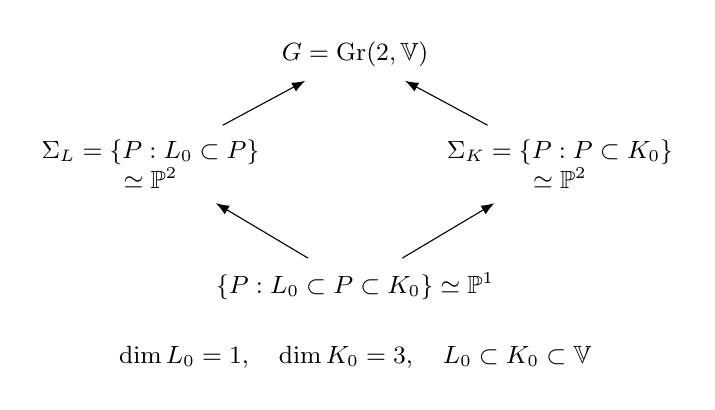
\begin{tikzpicture}[>=Latex, every node/.style={font=\small},
                    box/.style={align=center,inner sep=5pt}]
 \node[box] (g) at (0,2.8) {\(G=\Gr(2,\mathbb V)\)};
 \node[box] (l) at (-2.6,1.4)
   {\(\Sigma_L=\{P:L_0\subset P\}\)\\ \(\simeq\PP^2\)};
 \node[box] (k) at (2.6,1.4)
   {\(\Sigma_K=\{P:P\subset K_0\}\)\\ \(\simeq\PP^2\)};
 \node[box] (line) at (0,-0.15)
   {\(\{P:L_0\subset P\subset K_0\}\simeq\PP^1\)};
 \draw[->] (l) -- (g);
 \draw[->] (k) -- (g);
 \draw[->] (line) -- (l);
 \draw[->] (line) -- (k);
 \node[box] at (0,-1.05)
   {\(\dim L_0=1,\quad\dim K_0=3,\quad L_0\subset K_0\subset\mathbb V\)};
\end{tikzpicture}

 \caption{The Schubert line obtained from \(N=\tau N_0\).
 For the fixed incident flag \(L_0\subset K_0\), the two
 Schubert planes meet along this line. The chosen flat family
 has this line as its reduced central fibre inside the larger
 fibre \(G\). Arrows denote inclusions.}
 \label{fig:schubert}
\end{figure}
The directions are parametrized by flags
\(L_0\subset K_0\subset\mathbb V\); including the plane gives
\(L_0\subset P\subset K_0\).
Over \(S^\circ\), projective extension transitions are in
\(PGL_2\), so their action on the fibre's integral cohomology
is trivial. This does not trivialize the projective bundle.

The normal bundle of \(G\) is \(T^*G\).
Writing a cotangent vector as a map
\(\mathbb V/P\to P\), the preimage of the rank-at-most-one locus has
equation given by its \(2\times2\) determinant.
Its restriction line bundle is
\(\det P\otimes\det(\mathbb V/P)^*=\OO_G(-2h)\), where
\(h=c_1(\mathcal U)\). This records the incidence of the moving
exceptional divisor with the deep core.

\section{Schubert classes and the attachment modulo six}\label{sec:schubert}

Work first in the positive chamber, with the actual extension
\eqref{eq:actual-extension}. Write
\(h=c_1(\mathcal U)\), \(p=c_2(\mathcal U)\).
The integral Schubert presentation \cite[Section~3]{buch} is
\begin{equation}\label{eq:schubert-ring}
 H^*(G,\Z)=\Z[h,p]/(h^3-2hp,\ h^2p-p^2),\qquad
 |h|=2,\quad |p|=4,
\end{equation}
with
\begin{equation}\label{eq:schubert-evaluations}
 \int_G h^4=2,\qquad\int_G h^2p=\int_G p^2=1.
\end{equation}
The second degree-four Schubert class is \(q=h^2-p\);
thus \(\int_G q^2=1\) and \(\int_G pq=0\).
These are the classical two Schubert directions of \(\Gr(2,4)\).
They are represented by planes of the two types: planes containing
a fixed line, and planes contained in a fixed three-space.

\subsection{Removing the universal-family twist}
In the lattice embedding \eqref{eq:rankseven-lattice}, put
\(D=e-22f\). The integral Mukai vectors
\[
 x=(0,-f,0),\qquad y=(0,3f,1)
\]
are topological \(K\)-classes; algebraicity is not required.
Their Euler pairings are
\[
 \chi(A,x)=1,\quad\chi(B,x)=0,\qquad
 \chi(A,y)=0,\quad\chi(B,y)=1.
\]
If the restricted universal family differs from
\eqref{eq:actual-extension} by a line \(L\), then
\(I_x|_G=\mathcal U\otimes L\) and \(I_y|_G=L\).
The global virtual rank of \(I_y\) is one. Tensor the universal
class by \(\det(I_y)^{-1}\); this removes \(L\) on \(G\).
For the resulting normalized indices,
\begin{equation}\label{eq:index-restrictions}
 I_z|_G=m_z[\mathcal U]+n_z[1],\qquad
 c(I_z|_G)=(1+h+p)^{m_z},\qquad
 m_z=\chi(A,z),\quad n_z=\chi(B,z).
\end{equation}
The binomial expansion is integral for every integer \(m_z\),
including negative ones.

In particular \(c_1(I_x)\) and \(c_2(I_x)\) extend \(h,p\)
integrally to \(M\). Since \(h,p\) generate
\eqref{eq:schubert-ring}, restriction is onto in every degree.
Duality makes every corresponding inclusion
\(H_k(G,\Z)\to H_k(M,\Z)\) primitive.
The class \([G]\) is primitive because the integral extension
\(c_2(I_x)^2\) evaluates to one on it.
This is stronger than the information from divisors:
every divisor restricts to a multiple of \(h\), whose fourth
power has evaluation two.

\subsection{The boundary and complement}
The Plücker embedding identifies \(G\) with a smooth quadric
fourfold in \(\PP^5\). The Euler and normal sequences give
\[
 c(TG)=\frac{(1+h)^6}{1+2h},\qquad
 c_4(TG)=3h^4=6p^2 .
\]
Since \(G\) is Lagrangian, its normal bundle is \(T^*G\), so
\begin{equation}\label{eq:self-intersection}
 [G]^2=\int_G c_4(T^*G)=6 .
\end{equation}
For the boundary \(L=S(T^*G)\), the sphere-bundle Gysin sequence
and \eqref{eq:schubert-ring} give
\begin{equation}\label{eq:boundary-groups}
 H^j(L,\Z)=
 \begin{cases}
 \Z,&j=0,2,6,9,13,15,\\
 \Z^2,&j=4,11,\\
 \Z/6,&j=8,\\
 0,&\text{otherwise}.
 \end{cases}
\end{equation}
The only nonzero Euler multiplication is from degree zero
to degree eight, where it is multiplication by six.
This is a smooth boundary of the resolved neighborhood;
the target has a six-dimensional singular stratum through \(o\),
so it is not the link of an isolated singularity.

Put \(V=M\setminus G\). Markman's theorem gives torsion-free even
cohomology of \(M\), and the primitive inclusions just proved
make the relative sequence torsion-free. More explicitly,
\(H^k(M,V;\Z)=H_{16-k}(G,\Z)\); its map to \(H^k(M,\Z)\)
is the dual of restriction and is a primitive injection whenever
nonzero. Odd groups of \(V\) vanish. The classical \(X^{[4]}\)
Betti numbers, obtained from Göttsche's formula \cite{gottsche},
therefore give
\[
\begin{array}{c|rrrrrrrrr}
k&0&2&4&6&8&10&12&14&16\\ \hline
\rank H^k(M)&1&23&300&2852&19298&2852&300&23&1\\
\rank H^k(V)&1&23&300&2852&19297&2851&298&22&0 .
\end{array}
\]
The ranks removed in degrees \(8,10,12,14,16\) are
\(1,1,2,1,1\). These ranks do not by themselves give the
marked complement ring needed for attachment.

\subsection{The calculated congruence}
Apply Theorem~\ref{thm:attachment} with \(n=8\),
\(\Lambda=\Z[G]\) and \(B=(6)\).
For a marked universal-index Chern monomial of degree eight
on \(V\), substitute \eqref{eq:index-restrictions}, reduce by
\eqref{eq:schubert-ring}, and evaluate using
\eqref{eq:schubert-evaluations}, modulo six.
This specifies a homomorphism
\(\kappa:H^8(V,\Z)\to\Z/6\) on all integral generators.
In detail, for \(m=m_z\),
\begin{equation}\label{eq:chern-polynomials}
 \begin{aligned}
 c_1(I_z)|_G&=mh,\\
 c_2(I_z)|_G&=mp+\binom m2h^2,\\
 c_3(I_z)|_G&=\frac{m(m^2-1)}3\,hp,\\
 c_4(I_z)|_G&=\frac{m^2(m^2-1)}{12}\,p^2 .
 \end{aligned}
\end{equation}
The displayed coefficients are integer-valued for every integer
\(m\). The ring relations give the rule for all products, including
products involving different indices. The all-relations argument
in Theorem~\ref{thm:attachment} proves that this calculation
depends only on the specified complement class.

We obtain the explicit integral reconstruction
\begin{equation}\label{eq:mod-six}
 H^8(M,\Z)\simeq
 \{(u,N)\in H^8(V,\Z)\oplus\Z:
                  N\equiv\kappa(u)\pmod6\}.
\end{equation}
Moreover
\(\kappa(c_2(I_x)^2|_V)=1\), so \(\kappa\) is onto.
The higher index class supplies the odd evaluation which fourth
powers of divisor classes cannot supply. Both Schubert directions,
and their integral attachment, are thus visible in the same
compact moduli family.

For the negative chamber the pure extension axis instead restricts
the normalized universal class to \(A\boxtimes\mathcal S+B\),
where \(\mathcal S\) is the tautological subbundle in the
image-of-\(Y_1\) description. Its Chern classes
\(c_1(\mathcal S)=-h\), \(c_2(\mathcal S)=q=h^2-p\)
again generate the full integral ring. The same duality argument
proves all primitive inclusions in that chamber as well.

The core is also genuinely different from a toric core component.
Indeed \(\Pic(G)=\Z h\), so a connected automorphism preserves the
Plücker embedding and acts through the projective orthogonal group
of its smooth quadric. Its maximal torus has dimension three.
A dense torus action on a toric fourfold would require dimension
four. This observation is not needed for \eqref{eq:mod-six};
the two independent Schubert classes already explain the extra
integral information.

\section{Harmonic geometry of the same cycles}\label{sec:cycle-metrics}

The integral identification now determines exact metric periods.
Ambient diameters require an additional argument, because a shortest
path between points of an exceptional cycle may leave it.

\subsection{Periods and primitive curve classes}
For \(z\in v^\perp\), the normalized extension gives
\[
 \theta_v(z)|_G=-(a,z)h .
\]
Thus a positive minimal line \(\ell\) represents the functional
\(-a\) on \(v^\perp\). Since \((a,v)=0\), its
Beauville--Bogomolov square is \(-2\).
The integral vector \(z_0=(0,-7f,-2)=x-2y\) satisfies
\((v,z_0)=0\), \((a,z_0)=-1\); its Mukai class restricts to
\(h\), proving primitivity of \(\ell\) directly.
The proper family \eqref{eq:line-specialization}, rather than
divisor pairings alone, identifies the moving fibre class with
this line class.

For \(t>0\), put
\begin{equation}\label{eq:kappa-scale}
 \kappa_t=\frac{88\pi t}{7},\qquad
 b_t=(0,H+tD,-88t/7).
\end{equation}
We have \((a,b_t)=-44t/7\), so
\eqref{eq:harmonic-class} gives the exact formulas
\begin{equation}\label{eq:cycle-volumes}
 \begin{gathered}
 \operatorname{Area}_{g_t}(\ell)=\operatorname{Area}_{g_t}(f)
       =\pi\kappa_t,\\
 \Vol_{g_t}(\PP^2)=\frac{(\pi\kappa_t)^2}{2},\qquad
 \Vol_{g_t}(G)=\frac{(\pi\kappa_t)^4}{12}.
 \end{gathered}
\end{equation}
Either Schubert plane type is allowed. Its \(h^2\)-integral is
one; the \(h^4\)-integral on \(G\) is two.
These are Kähler volume identities on the actual holomorphic
cycles, not a claim that the induced metric is exactly homogeneous.
For \(t<0\), set \(\kappa_t=88\pi|t|/7\) and reverse the
extension convention. The effective line functional is then
\(+a\) in that chamber's Mukai marking, and the positive
formulas are unchanged.

\subsection{A distance-preserving zero section}
Consider the positive-level complete quotient
\[
 Z_1Y_1=0,\qquad Z_1Z_1^*-Y_1^*Y_1=\kappa I_2
\]
with the flat Hilbert--Schmidt metric. Let \(g_{\Gr}\) denote
the homogeneous Grassmannian metric with minimal line area
\(\pi\).

\begin{lemma}\label{lem:grass-retraction}
The projection to \(\ker Z_1\) is a 1-Lipschitz retraction of the
quotient onto its zero section with metric \(\kappa g_{\Gr}\).
Consequently the ambient distances between core points equal
their intrinsic Grassmannian distances. In the unit normalization,
\[
 \diam G=\frac{\pi}{\sqrt2},\qquad
 \diam \PP^2=\frac{\pi}{2}
\]
for either Schubert plane, with ambient distances in the
complete quotient.
\end{lemma}

\begin{proof}
The real moment equation gives \(Z_1Z_1^*\ge\kappa I_2\).
Let \(P_{\rm row}\) be the orthogonal projector onto the row
space of \(Z_1\).
The horizontal derivative of its row-space orthonormal frame
has the form
\((I-P_{\rm row})\delta Z_1^*(Z_1Z_1^*)^{-1/2}\).
The equivalent kernel description therefore satisfies
\[
 \kappa\,|d(\ker Z_1)|_{g_{\Gr}}^2
       \le\|\delta Z_1\|^2
       \le\|\delta Z_1\|^2+\|\delta Y_1\|^2.
\]
The projection kills vertical orbit directions, so this bound
survives minimization defining the quotient norm.
On \(Y_1=0\), the equation \(Z_1Z_1^*=\kappa I_2\) gives
the Stiefel quotient metric \(\kappa g_{\Gr}\).
The retraction is the identity there; the inclusion and
retraction prove equality of the two distances.

For two planes, use principal vectors to rotate the two
orthogonal blocks through angles
\(\theta_1,\theta_2\in[0,\pi/2]\).
The horizontal frame path has length
\(\sqrt{\theta_1^2+\theta_2^2}\le\pi/\sqrt2\).
For orthogonal planes, each column of any horizontal frame
lift travels spherical distance at least \(\pi/2\).
Minkowski's integral inequality bounds its Hilbert--Schmidt
length below by \(\pi/\sqrt2\), proving sharpness.
For either Schubert plane all planes share a fixed line or
lie in a fixed three-space; one principal angle vanishes.
The same argument gives diameter \(\pi/2\) and the induced
line-area-\(\pi\) Fubini--Study metric: the principal-vector
path gives the upper bound. For the lower bound take
\(P=\langle e_1,e_2\rangle\) and
\(P'=\langle e_1,e_3\rangle\) in either Schubert plane type.
In a horizontal frame lift starting at \((e_1,e_2)\), the second
column ends in \(P'\), orthogonal to \(e_2\), and so travels
spherical distance at least \(\pi/2\). The Hilbert--Schmidt
length dominates that column length.
\end{proof}

The complete cotangent Grassmannian metric is classical
\cite[Theorem~1 and Section~2.2]{biquardgauduchon}.
The retraction argument above verifies the ambient-distance
statement needed for its transfer to the compact moduli.

\begin{proposition}\label{prop:actual-diameters}
In the actual eightfold, for either chamber,
\begin{equation}\label{eq:actual-diameters}
 \diam_{M,g_t}G=\frac{\pi}{\sqrt2}\sqrt{\kappa_t}\,
                  (1+O(|t|)),\qquad
 \diam_{M,g_t}\PP^2=\frac{\pi}{2}\sqrt{\kappa_t}\,
                  (1+O(|t|)).
\end{equation}
After distances are divided by \(\sqrt{\kappa_t}\), the ambient
spaces based on \(G\) converge in complete pointed
Gromov--Hausdorff topology to the unit-level \(T^*\Gr(2,4)\)
quotient. Along compact subsets of \(S^\circ\), the moving fibre
has transverse Eguchi--Hanson limit and
\[
 \diam_{M,g_t} f/\sqrt{\kappa_t}\longrightarrow\pi/2
\]
uniformly.
\end{proposition}

\begin{proof}
The deepest finite core has coefficient norm squared \(2\kappa_t\).
Finite competitors have length \(O(\sqrt{\kappa_t})\), and
their actual images have that length bound. The first-exit
cost from a fixed larger chart stays positive. An actual
near-minimizer cannot leave it; the 1-Lipschitz finite radius
and coarse metric bound then keep such a path in coefficient
radius \(O(\sqrt{\kappa_t})\).
On this smaller region \eqref{eq:relative} has error \(O(|t|)\).
It therefore compares both ambient distance infima, not merely
the tensors on the core. Lemma~\ref{lem:grass-retraction} gives
\eqref{eq:actual-diameters}.

After rescaling, fixed chart domains exhaust the entire finite
quotient. Exit barriers diverge, relative errors tend to zero
on every bounded model ball, and inverse coverage supplies the
whole corresponding actual ball. Finite intrinsic continuity
then gives the complete pointed limit. The unitary symmetry is
transitive on the core, so any choice of core basepoint gives
the same pointed limit up to isometry.

Fix a compact subset \(K\subset S^\circ\) and an accuracy
\(\epsilon>0\). At each point choose a full \(\C^6\) times
two-arrow quotient chart, with nested inner and outer domains,
so small that the \(\|x\|^2\) term in \eqref{eq:relative}
is below \(\epsilon\) on the outer domain. Cover \(K\) by
finitely many inner domains, as in Proposition~\ref{prop:coverage},
and then choose \(|t|\) small enough for all parameter errors
to be below \(\epsilon\) and for whole-fibre coverage to hold.
The normal zero sections are the moving projective lines,
with the same level \(\kappa_t\). Competitors of length
\(O(\sqrt{\kappa_t})\) cannot cross the positive outer exit
barriers. Projection to the normal zero section therefore gives,
uniformly over \(K\), the ratio \(\pi/2\) with a relative
error \(O(\epsilon)\). Let \(t\to0\) first and then
\(\epsilon\to0\).

The same choice works on any prescribed bounded rescaled ball.
The outer exit costs diverge after rescaling, and inverse
coverage supplies all actual points of the ball. Translating
the trivial coordinates to the moving center gives the full
pointed limit \(\C^6\) times the unit-level Eguchi--Hanson
space; its transverse factor is the asserted limit.
\end{proof}

\subsection{Successive scales with moving centers}\label{subsec:successive}
The following proposition also covers basepoints approaching a
deeper stratum.

\begin{proposition}\label{prop:successive-limits}
Assume \textup{(G1)--(G3)}.
Fix a central chart at \(p\), numbers \(\delta_n\downarrow0\),
and generic parameters \(\theta_n\to0\).
Suppose
\[
 \nu_n=\zeta_p(\theta_n)/\delta_n^2\longrightarrow\nu,
 \qquad x_n\longrightarrow x
\]
for balanced representatives \(x_n\) at level \(\nu_n\),
after unitary adjustment. Then
\begin{equation}\label{eq:first-rescaling}
 (M_{\theta_n},\delta_n^{-1}d_{\theta_n},
               f_{p,\theta_n}([\delta_nx_n]))
 \longrightarrow(Q_\nu,d_\nu,[x])
\end{equation}
in complete pointed Gromov--Hausdorff topology.

For a further scale, retain a limiting representative \(x_*\)
and its compact stabilizer \(K_*\).
Write its full normal representation as
\(W=T\oplus W'\), where \(T=W^{K_*}\) and
\(W'=T^\perp\) for the invariant hyperk\"ahler inner product.
In the common slice suppose the current representatives are
\((u_n,z_n)\to0\). For \(\sigma_n\downarrow0\), require
\begin{equation}\label{eq:successive-data}
 \frac{(\nu_n-\nu)|_{\Lie K_*}}{\sigma_n^2}\longrightarrow\lambda,
 \qquad \frac{z_n}{\sigma_n}\longrightarrow z_* .
\end{equation}
At physical scale \(\delta_n\sigma_n\), the complete pointed
limit is
\[
 T\times(W'\!/\!/\!/_\lambda K_*),\qquad
 \text{based at }(0,[z_*]).
\]
The notation \( /\!/\!/_\lambda\) means complex moment zero
and real moment \(\lambda\).
Tangential motion \(u_n\) need only tend to zero; it need not
be comparable with \(\sigma_n\).
This rule can be repeated for every fixed finite number of
stages, retaining each stabilizer, full normal representation,
normalized level and normal basepoint.
\end{proposition}

\begin{proof}
On a bounded region \(\|x\|\le R\) of the first rescaled
finite model, \eqref{eq:relative} has squared-metric error
\(O_p(|\theta_n|+\delta_n^2R^2)=o(1)\).
The fixed outer chart has a positive first-exit cost by
\eqref{eq:exit}; divided by \(\delta_n\), this tends to infinity.
Its coarse comparison and the 1-Lipschitz model radius keep
every bounded-length rescaled actual path in a bounded model
region. Conversely bounded model competitors scale into the
chart. Proposition~\ref{prop:coverage} and the inverse local
solution chart give entire actual balls. Thus both ambient
distance infima are compared. The finite intrinsic continuity
theorem \cite[Theorem~5.1]{wuebben14}, applicable by (G3), now
gives \eqref{eq:first-rescaling}.

For the next scale apply the full normal metric slice and
moving-center results \cite[Sections~4,6]{wuebben14} in this
finite model. After \((u,z)=(u_n+\sigma_n u',\sigma_n z')\),
their error on a bounded normal ball is
\[
 O_{x_*}(|\nu_n-\nu|+|u_n|+\sigma_n R)=o(1).
\]
Translation in the fixed subspace removes \(u_n\) without
changing the moment equations. The outer harmonic error is
multiplicative and is not divided by \(\sigma_n\).
Both the outer chart and a fixed inner slice have divergent
exit costs at physical scale \(\delta_n\sigma_n\).
The same two-sided path comparison and inverse coverage
therefore identify the entire complete product limit stated above.
Full normal slices retain the simple-zero hypothesis
\cite[Lemma~6.3]{wuebben14}. For any fixed finite iteration,
the relative errors sum to \(o(1)\), and the nested exit
barriers give coverage at each physical scale. This proves
the result directly from (G1)--(G3).
\end{proof}

In the eightfold, a rank-one point of the zero cone has full
normal model \(\C^6\) times the \(A_1\) quotient.
Thus approaching the deepest point is handled by the \(U(2)\)
model first, followed, when appropriate, by this full slice.
No single limit is assigned to oscillating normalized data,
and no infinite iteration is asserted.

\begin{proof}[Proof of Theorem~\ref{thm:main}]
Section~\ref{sec:construction} constructs the surface, the unique
spherical bundle, both compact chamber spaces and their common
normal target. Lemma~\ref{lem:rank-list} and the compactness
argument exclude all additional ideal boundary; the whole-fibre
and target arguments identify every stratum and fibre.
The proper family in Section~\ref{subsec:specialization}
proves reduced integral specialization.
Section~\ref{sec:schubert} gives the primitive inclusions,
self-intersection and calculated mod-six attachment.
Equations~\eqref{eq:cycle-volumes} and
\eqref{eq:actual-diameters}, with
Proposition~\ref{prop:actual-diameters}, give the cycle metric
claims. The construction verifies (G1)--(G3), so
Proposition~\ref{prop:central-completion} and
Theorem~\ref{thm:quantitative} identify the harmonic completion
and control the full compact contraction graph.
\end{proof}

\section{Fourfold examples and the role of monodromy}\label{sec:examples}

\subsection{The isolated and interacting plane contractions}
The compact fourfolds in \cite{wuebben17} provide two further
applications of the general theorem. We verify its local
simple-zero hypothesis explicitly and record the additional
global metric conclusion; their construction and detailed cycle
geometry remain in that paper.

For the isolated example, the lattice is
\(\NS(X)=\Z H\oplus\Z D\) with Gram matrix
\(\operatorname{diag}(2,-22)\), and
\[
 a=(1,0,1),\quad b=(2,D,-5),\quad v=a+b.
\]
The compact chamber spaces have a single \(\PP^2\) fibre.
The complete factor list and no-charge theorem
\cite[Section~3]{wuebben17} verify (G1)--(G2).
The full deep representation is
\(\C^3\oplus(\C^3)^*\) under \(U(1)\), with complex equation
\(y(x)=0\). The point \(x=e_1,y=e_2^*\) is module-simple,
as both arrow directions between the two one-dimensional
vertices are nonzero. At stable points the effective group
is trivial. The convergent charts and classifying diagram
verify (G3).

For the interacting example, the lattice matrix and vectors are
\[
 \begin{pmatrix}2&0&0\\0&-6&-4\\0&-4&-8\end{pmatrix},\qquad
 a_0=(1,0,1),\quad a_1=(1,D_1,-2),\quad a_2=(1,D_2,-3),
 \quad v=a_0+a_1+a_2 .
\]
For \([\omega]=H+sD_1+tD_2\), the levels are
\[
 \zeta(s,t)=\frac{2\pi}{3}
 \begin{pmatrix}-10&-12\\8&0\\2&12\end{pmatrix}
 \binom{s}{t}.
\]
All six chamber spaces, their common normal target, complete
factor and charge lists, and whole fibres are constructed in
\cite[Sections~4--5]{wuebben17}. They verify (G1)--(G2).
At the deepest point the full effective group is
\(U(1)^3/U(1)\), with paired arrow dimensions \(1,2,1\).
In the coordinates of that paper,
\[
 zz'-\varphi(u)=ww'+\varphi(u)=0
\]
has the solution \(z=z'=w=1,\ w'=-1,\ u=\varphi=(1,0)\).
Its directed support is strongly connected, which for
one-dimensional vertices forbids a proper submodule.
Along the moving stratum the full representation is
\(\C^2\) times the two-arrow \(U(1)\) model, which has
the simple point \(e_1,e_2^*\); stable centers are smooth.
Together with the convergent classifying diagrams this verifies
(G3) on every stratum.

Theorem~\ref{thm:quantitative} consequently gives graph distortion
tending to zero in both examples, with the variational bound
\eqref{eq:global-distortion}. For the interacting family this
holds through all chamber directions and arbitrary ratios of
positive scales. It supplements the qualitative global
convergence of \cite{wuebben17} by a proof from the finite
quotient distances.

Their integral formulas are instances of
Theorem~\ref{thm:attachment}, with the explicit normalized
index restrictions already proved in
\cite[Proposition~6.1]{wuebben17}.
For the plane, \(B=(3)\) and
\[
 \kappa(c_2(I_z)|_V)=\binom{m_z}{2},\qquad
 \kappa(c_1(I_z)c_1(I_{z'})|_V)=m_zm_{z'}\pmod3.
\]
Here \(m_z\) is the Euler pairing with the extension subobject.
In the two-plane chamber, \(E=P_0\cup P_2\) and
\[
 B=\begin{pmatrix}3&1\\1&3\end{pmatrix},\qquad
 \coker B\simeq\Z/8,\qquad (n_0,n_2)\longmapsto n_0-3n_2 .
\]
With \(m_{i,z}=\chi(a_i,z)\), the boundary map is
\[
 \begin{aligned}
 \kappa(c_2(I_z)|_V)
   &=\binom{m_{0,z}}2-3\binom{m_{2,z}}2,\\
 \kappa(c_1(I_z)c_1(I_{z'})|_V)
   &=m_{0,z}m_{0,z'}-3m_{2,z}m_{2,z'}\pmod8 .
 \end{aligned}
\]
These formulas use the marked complement ring and respect all
its relations. The mod-eight statement concerns this
two-plane chamber. The other four configurations are not
assigned its global formula.

The proper moving-line family specializes as \(f=c_0+c_2\),
with both multiplicities one. For levels
\(\zeta_0=a>0,\zeta_2=b>0\), the exact areas are
\(\pi a,\pi b,\pi(a+b)\); the plane volumes are
\((\pi a)^2/2,(\pi b)^2/2\).
The ambient collapse and complete separated-scale limits are
those of \cite[Section~8]{wuebben17}, with unchanged metric
normalization. Thus the general global comparison and the
explicit attachment refer to those same cycles.

\subsection{The Schubert involution}
The following topological example explains why the geometric
transition information in Section~\ref{subsec:retained} cannot
be replaced by local fibre rings and divisor classes.

Choose a nondegenerate symmetric complex bilinear form on
\(\C^4\). Orthogonal complementation defines a holomorphic
involution \(\delta(P)=P^\perp\) of \(G=\Gr(2,4)\).
For its tautological subbundle \(\mathcal S\) and quotient
\(\mathcal U\), one has
\(\delta^*\mathcal S\simeq\mathcal U^*\). Consequently
\[
 \delta^*h=h,\qquad \delta^*p=q,\qquad \delta^*q=p .
\]
Form the compact smooth mapping tori \(T_1\) and \(T_\delta\)
over \(S^1\). Both have the same local product geometry,
integral fibre ring, and distinguished divisor class \(h\).
Their degree-four cohomology is different:
\begin{equation}\label{eq:monodromy}
 H^4(T_1,\Z)=\Z^2,\qquad H^4(T_\delta,\Z)=\Z .
\end{equation}
Indeed \(H^3(G,\Z)=0\), so the Wang sequence identifies
degree-four cohomology with the invariant subgroup of
\(H^4(G,\Z)=\Z p\oplus\Z q\). For the identity it is all of
that group; for \(\delta\) it is \(\Z(p+q)\).

This is a topological necessity example, not a claim that
the involution occurs in the K3 family above. It shows that
forgetting monodromy can change even a Betti number.
The use of all multiple intersections has a further purpose:
cochains retain their restriction maps and higher compatibility,
which fibre cohomology alone generally discards.
Theorem~\ref{thm:attachment} gives a smaller calculation only
under its explicit vanishing, intersection and generator
hypotheses.

The results concern compact K3 bundle-moduli contractions
without bubbling. Extending them to positive-charge strata
requires new local geometric and metric inputs. The
reconstruction of underlying degenerating manifolds and
unrestricted Hermitian--Yang--Mills dynamics are likewise
separate questions.

\begin{thebibliography}{Wue26c}

\bibitem[AS18]{arbarellosacca}
E. Arbarello and G. Sacc\`a,
\emph{Singularities of moduli spaces of sheaves on K3 surfaces and
Nakajima quiver varieties}, Adv. Math. \textbf{329} (2018), 649--703.
\href{https://doi.org/10.1016/j.aim.2018.02.003}{doi:10.1016/j.aim.2018.02.003}.

\bibitem[BMM21]{bmm}
R. Bandiera, M. Manetti and F. Meazzini,
\emph{Formality conjecture for minimal surfaces of Kodaira dimension 0},
Compos. Math. \textbf{157} (2021), 215--235.
\href{https://doi.org/10.1112/S0010437X20007605}{doi:10.1112/S0010437X20007605}.

\bibitem[BM14]{bayermacri}
A. Bayer and E. Macr\`i,
\emph{MMP for moduli of sheaves on K3s via wall-crossing: nef and
movable cones, Lagrangian fibrations}, Invent. Math. \textbf{198}
(2014), 505--590.
\href{https://doi.org/10.1007/s00222-014-0501-8}{doi:10.1007/s00222-014-0501-8}.

\bibitem[BG97]{biquardgauduchon}
O. Biquard and P. Gauduchon,
\emph{Hyperkähler metrics on cotangent bundles of Hermitian symmetric spaces},
in \emph{Geometry and Physics (Aarhus, 1995)},
J. E. Andersen, J. Dupont, H. Pedersen and A. Swann, eds.,
Lecture Notes in Pure and Appl. Math. \textbf{184},
Marcel Dekker, New York, 1997, 287--298.
\href{https://webusers.imj-prg.fr/~olivier.biquard/hs.pdf}{Author text}.

\bibitem[BS16]{biswasschumacher}
I. Biswas and G. Schumacher,
\emph{The Weil-Petersson current for moduli of vector bundles and
applications to orbifolds}, Ann. Fac. Sci. Toulouse Math. (6)
\textbf{25} (2016), no.~4, 895--917.
\href{https://doi.org/10.5802/afst.1514}{doi:10.5802/afst.1514}.

\bibitem[Buc17]{buch}
A. S. Buch,
\emph{Notes on Grassmannians}, class notes, Rutgers University,
4 September 2017.
\href{https://sites.math.rutgers.edu/~asbuch/notes/grass.pdf}{Author text}.

\bibitem[CB01]{crawleyboevey}
W. Crawley-Boevey,
\emph{Geometry of the moment map for representations of quivers},
Compos. Math. \textbf{126} (2001), 257--293.
\href{https://doi.org/10.1023/A:1017558904030}{doi:10.1023/A:1017558904030}.

\bibitem[Dri98]{vandendries}
L. van den Dries,
\emph{O-minimal structures and real analytic geometry},
Current Developments in Mathematics \textbf{1998}, no.~1,
International Press, 105--152.
\href{https://doi.org/10.4310/CDM.1998.v1998.n1.a4}{doi:10.4310/CDM.1998.v1998.n1.a4}.

\bibitem[G\"ot90]{gottsche}
L. G\"ottsche,
\emph{The Betti numbers of the Hilbert scheme of points on a smooth
projective surface}, Math. Ann. \textbf{286} (1990), 193--207.
\href{https://doi.org/10.1007/BF01453572}{doi:10.1007/BF01453572}.

\bibitem[GSTW21]{gstw}
D. Greb, B. Sibley, M. Toma and R. Wentworth,
\emph{Complex algebraic compactifications of the moduli space of
Hermitian--Yang--Mills connections on a projective manifold},
Geom. Topol. \textbf{25} (2021), 1719--1818.
\href{https://doi.org/10.2140/gt.2021.25.1719}{doi:10.2140/gt.2021.25.1719}.

\bibitem[GT17]{grebtoma}
D. Greb and M. Toma,
\emph{Compact moduli spaces for slope-semistable sheaves},
Algebr. Geom. \textbf{4} (2017), no.~1, 40--78.
\href{https://doi.org/10.14231/AG-2017-003}{doi:10.14231/AG-2017-003}.

\bibitem[Hat02]{hatcher}
A. Hatcher,
\emph{Algebraic Topology}, Cambridge University Press,
Cambridge, 2002.
\href{https://pi.math.cornell.edu/~hatcher/AT/ATpage.html}{Author text}.

\bibitem[HL10]{huybrechtslehn}
D. Huybrechts and M. Lehn,
\emph{The Geometry of Moduli Spaces of Sheaves}, 2nd ed.,
Cambridge Mathematical Library, Cambridge University Press,
Cambridge, 2010.
\href{https://doi.org/10.1017/CBO9780511711985}{doi:10.1017/CBO9780511711985}.

\bibitem[KS24]{kaplanschedler}
D. Kaplan and T. Schedler,
\emph{Crepant resolutions of stratified varieties via gluing},
Internat. Math. Res. Notices \textbf{2024}, no.~17, 12161--12200.
\href{https://doi.org/10.1093/imrn/rnae135}{doi:10.1093/imrn/rnae135}.

\bibitem[LS13]{lakziansormani}
S. Lakzian and C. Sormani,
\emph{Smooth convergence away from singular sets},
Comm. Anal. Geom. \textbf{21} (2013), no.~1, 39--104.
\href{https://doi.org/10.4310/CAG.2013.v21.n1.a2}{doi:10.4310/CAG.2013.v21.n1.a2}.

\bibitem[LS20]{lakziansormanier}
S. Lakzian and C. Sormani,
\emph{Errata to “Smooth convergence away from singular sets”},
Comm. Anal. Geom. \textbf{28} (2020), no.~7, 1755--1772.
\href{https://doi.org/10.4310/CAG.2020.v28.n7.e1}{doi:10.4310/CAG.2020.v28.n7.e1}.

\bibitem[Mar01]{markmanbn}
E. Markman,
\emph{Brill--Noether duality for moduli spaces of sheaves on K3 surfaces},
J. Algebraic Geom. \textbf{10} (2001), no.~4, 623--694.
\href{https://arxiv.org/abs/math/9901072}{arXiv:math/9901072}.

\bibitem[Mar07]{markman}
E. Markman,
\emph{Integral generators for the cohomology ring of moduli spaces
of sheaves over Poisson surfaces}, Adv. Math. \textbf{208} (2007),
no.~2, 622--646.
\href{https://doi.org/10.1016/j.aim.2006.03.006}{doi:10.1016/j.aim.2006.03.006}.

\bibitem[MM25]{matteimeinsma}
D. Mattei and R. Meinsma,
\emph{Obstruction classes for moduli spaces of sheaves and Lagrangian fibrations},
preprint, 21 July 2025.
\href{https://arxiv.org/abs/2404.16652v2}{arXiv:2404.16652v2}.

\bibitem[Mor84]{morrison}
D. R. Morrison,
\emph{On K3 surfaces with large Picard number},
Invent. Math. \textbf{75} (1984), 105--121.
\href{https://doi.org/10.1007/BF01403093}{doi:10.1007/BF01403093}.

\bibitem[Son14]{song}
J. Song,
\emph{Riemannian geometry of K\"ahler--Einstein currents},
preprint, 2014.
\href{https://arxiv.org/abs/1404.0445}{arXiv:1404.0445}.

\bibitem[Tos09]{tosatti}
V. Tosatti,
\emph{Limits of Calabi--Yau metrics when the K\"ahler class degenerates},
J. Eur. Math. Soc. (JEMS) \textbf{11} (2009), no.~4, 755--776.
\href{https://doi.org/10.4171/JEMS/165}{doi:10.4171/JEMS/165}.

\bibitem[Wue26a]{wuebben14}
B. J. Wuebben,
\emph{Quantitative metric wall crossing for K3 bundle moduli},
6 November 2026.
\href{https://doi.org/10.5281/zenodo.24024998}{doi:10.5281/zenodo.24024998}.

\bibitem[Wue26b]{wuebben15}
B. J. Wuebben,
\emph{Quantitative local models for Hermitian--Einstein metrics},
7 November 2026.
\href{https://doi.org/10.5281/zenodo.24029090}{doi:10.5281/zenodo.24029090}.

\bibitem[Wue26c]{wuebben17}
B. J. Wuebben,
\emph{Exceptional cycles and harmonic metrics in K3 bundle moduli},
7 November 2026.
\href{https://doi.org/10.5281/zenodo.24046092}{doi:10.5281/zenodo.24046092}.

\bibitem[Yos00]{yoshioka99}
K. Yoshioka,
\emph{Irreducibility of moduli spaces of vector bundles on K3 surfaces},
preprint, 2000.
\href{https://arxiv.org/abs/math/9907001v2}{arXiv:math/9907001v2}.

\bibitem[Yos01]{yoshioka01}
K. Yoshioka,
\emph{Moduli spaces of stable sheaves on abelian surfaces},
Math. Ann. \textbf{321} (2001), 817--884.
\href{https://doi.org/10.1007/s002080100255}{doi:10.1007/s002080100255}.

\end{thebibliography}

\bigskip
\noindent{\sc Bernd Johannes Wuebben, New York, NY,}
\texttt{wuebben@gmail.com}
\end{document}
